%!TEX root = ../../dissertation.tex
%%%%%%%%%%%%%%%%%%%%%%%%%%%%%%%%%%%%%%%%%%%%%%%%%%%%%%%%%%%%%%%%%%%%%%%%%%%%%%%%
\section{Mobile Network Architecture}
\label{c4:sec:3gpparchitecture}

Today's dominating commercial mobile network system, which includes \gls{GSM}, \gls{UMTS}, and up to \gls{LTE}, is designed and specified by the \gls{3GPP}. This group is an umbrella organization for several standardization bodies, including the European \gls{ETSI} and their individual members --- in this case mostly telecommunication companies. Unlike the \gls{IETF}, the Internet's de facto standards body, natural persons cannot participate in the \gls{3GPP} on their own but only through the organizational members.

Specifications are not released individually but are instead grouped together into larger releases once every or every other year. \gls{GSM} was first specified in the \textit{Phase 1} release in 1992 with \gls{GPRS} added in \textit{Release 97} (1998). \gls{UMTS} followed with \textit{Release 99} (2000), but most \gls{3G} networks operate at least with \textit{Release 5} (2002), \textit{Release 6} (2004), or \textit{Release 7} (2007) as they introduced \gls{HSDPA}, \gls{HSUPA}, and \gls{HSPA+} likewise. \gls{LTE} first found its way into the specifications in 2008 with \textit{Release 8}. \textit{Release 12} is scheduled to be published in March of 2015. This background section mostly describes the \gls{UMTS} based \gls{TS} with some comparisons being made to the older \gls{GPRS} and the latest \gls{LTE} specification versions where available.

\begin{figure}[htbp]
	\centering
	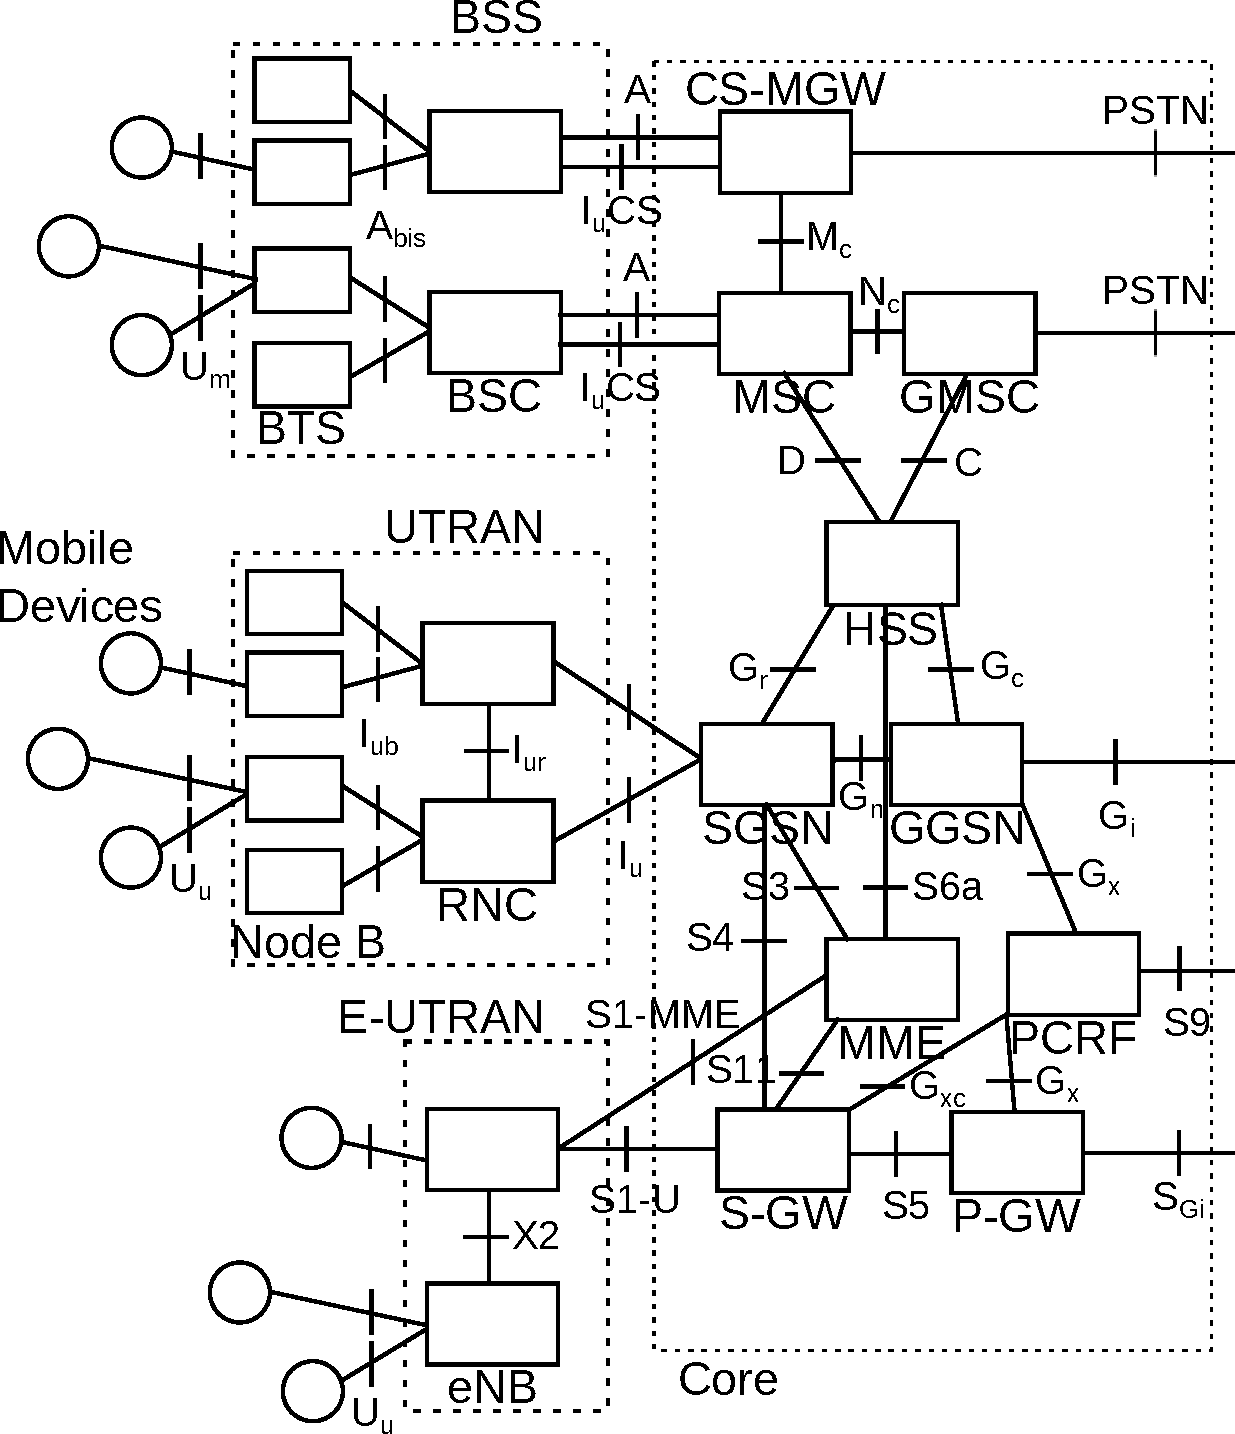
\includegraphics[width=0.9\textwidth]{images/3gpp-physical-arch.pdf}
	\caption{Overview of a combined \gls{CS}/\gls{PS} \gls{GSM}/\gls{UMTS}/\gls{LTE} architecture.}
\label{c4:fig:psdomain}
\end{figure}

Today's most common version of the mobile network architecture is depicted in Figure~\ref{c4:fig:psdomain} and based on \gls{3GPP} \gls{TS} 23.002~\cite{3gpp.23.002}, with some minor nodes and network paths omitted\footnote{For a complete reference of all the acronyms and addressing schemes used in \gls{3GPP} specs please refer to \gls{TS} 21.905~\cite{3gpp.21.905} and \gls{TS} 23.003~\cite{3gpp.23.003}}. The displayed architecture combines all three access technologies as well as the \gls{CS} and the \gls{PS} domains of the core. 

Concerning the \gls{PS} domain, one has to further distinguish between links and nodes used solely for control plane tasks as well as links and nodes that are in path of the actual user \gls{IP} traffic. For \gls{UMTS} and \gls{GPRS}\footnote{\gls{GPRS} provides \gls{PS} data services for \gls{GSM} radio access. The same core infrastructure is also used in the \gls{UMTS} \gls{PS} domain.} the \gls{SGSN} and the \gls{GGSN} are the core elements inside the user traffic path. Everything else solves just control plane tasks.

One thing to keep in mind is the strict separation between user plane and control plane tasks in the \gls{3GPP} architecture. Here completely separate protocol stacks are used and signaling is mostly conducted in an explicit and out of band manner. This is contrary to the typical approach of the Internet's \gls{TCP}/\gls{IP} stack, especially its upper layers, where most state is implicitly inferred and only some signaled in-band. 

The following sections give a short description of nodes and their tasks as well as used protocols stacks and signaling procedures for both the user and the control plane. The description will be mostly focused on the \gls{UMTS} parts of the architecture which is also overviewed in \cite{3gpp.23.101}.


%%
\subsection{\texorpdfstring{\acrshort{3GPP}}{3GPP} Radio Network}

The architecture has three completely distinct radio networks, one for each access technology: \gls{GSM}'s \gls{BSS} (or more complete: \gls{GERAN}), \gls{UTRAN} for \gls{UMTS}, and \gls{E-UTRAN} in \gls{LTE}.

Essential to the radio network is a base station, a radio transceiver providing the physical connection to the user's mobile device\footnote{Mobile devices are called \gls{MS} in \gls{GSM} networks and \gls{UE} in \gls{3G} and later.} \gls{3G}'s base station is called \textit{Node B}. The used radio spectrum is divided into a number of channels, with various shared channels responsible for management and control plane signaling and one or more dedicated channel for each active mobile device~\cite{3gpp.25.201,3gpp.25.301}. Layer 2 consists of several protocols managing and multiplexing transmissions on the link. These are \gls{MAC}~\cite{3gpp.25.321} and \gls{RLC}~\cite{3gpp.25.322} with an additional user plane broadcast service provided by \gls{BMC}~\cite{3gpp.25.324}. 

On layer 3, the actual radio control plane signaling protocol \gls{RRC}~\cite{3gpp.25.331} resides, managing the device's state and the radio connection. Some of the signaling procedures are detailed in \cite{3gpp.25.931}. Additionally, \gls{PDCP}~\cite{3gpp.25.323} provides the connection to the  usual Internet \gls{TCP}/\gls{IP} user plane stack atop. Thus, all user traffic is encapsulated into so called \textit{radio bearers}, which tunnels traffic from the mobile device directly into the core network.

Each base station acts as an independent radio cell. Mobile devices can be seamlessly handed over between cells without higher layers being able to notice this.\footnote{However, there are still many ways to detect a handover in the upper layers of a mobile device.} The handover process is fully controlled and conducted by the network through a node that shares the old and new path to the device. For \gls{UMTS}, in most cases this can be handled by the \gls{RNC} while the core \gls{SGSN} is responsible for handovers between larger regions.

In \gls{UMTS} multiple Node B are concentrated into one \gls{RNC}. Most of the functions of a \gls{RNC}, including \gls{MM}, are defined by the \gls{RANAP} control plane protocol defined in \cite{3gpp.25.413}. \gls{RANAP} is used at the Iu interface between the \gls{RNC} and the core network, i.e., the \gls{SGSN}. Today, all non-radio links of the network are usually \gls{IP}-based. But in the past all interfaces have also been explicitly defined for \gls{ATM} and exhibited some differences to their \gls{IP}-based counterparts. The connection of the decentralized parts of the radio network to either the core network itself or a \gls{RNC} is called \textit{backhaul}. This term usually subsumes the bulk transport of data over dedicated links to a central location. Often, optical fiber or microwave transmission links are used.


%%
\subsection{\texorpdfstring{\acrshort{3GPP}}{3GPP} Core Network}

The \gls{PS} domain of a mobile core network manages most of the aspects of the connected devices and acts as the bridge and gateway to the Internet. It consists of nodes that are directly in the path of the user plane traffic as well as additional nodes, that only exist in the control plane.

\gls{GPRS} and \gls{UMTS} use the exact same \gls{PS} core network architecture. Only \gls{LTE} introduced a new core network concept, the \gls{EPC}. If one core has to simultaneously provide support for both \gls{UMTS} and \gls{LTE} access, core nodes for both architectures have to be present. The exception are some \gls{EPC} nodes that provide legacy interfaces to supplant their \gls{UMTS} predecessors.

The two central elements in the user plane's path are the \gls{SGSN} and the \gls{GGSN}~\cite{3gpp.22.060,3gpp.23.060}. The \gls{SGSN} is the endpoint of the \gls{RAB}, tunneling user traffic from the \gls{UE} to the core, and an endpoint for the \gls{gtp} based core tunnel, further transporting user plane traffic to the \gls{GGSN}. \Gls{gtp} will be described in detail in Section~\ref{c4:sec:gtp}. The \gls{GGSN}'s control plane tasks include mobility and connection management via \gls{RANAP} to the \gls{RNC}. The necessary information is cached and retrieved from the \gls{HLR} using \gls{MAP}~\cite{3gpp.29.002}. The \gls{HLR} or, respectively, the \gls{HSS} in an \gls{EPC}, acts as the central storage of all the operator's subscriber information.

The \gls{GGSN} represents the gateway to the public Internet and therefore typically is the only node in the network, that has a publicly routable \gls{IP} address. It filters incoming traffic into the corresponding \gls{gtp} tunnel and routes packets to the correct \gls{SGSN}. State about any active tunnel and device has to be kept locally and is initially retrieved from the \gls{SGSN}.

In \gls{EPC} user traffic in the core is handled by the \gls{SGW} and \gls{PGW}, having similar functions as their \gls{GPRS} counterparts \gls{SGSN} and \gls{GGSN}. Depending on the specific version of the implemented infrastructure these two nodes can also be combined into one, eliminating the S5 interface and the \gls{gtp} signaling between them. Much of the control plane tasks of the \gls{SGSN} have now been offloaded to a new node, the \gls{MME}, which maintains its own logical connection to the radio network using the \gls{S1AP} signaling protocol~\cite{3gpp.36.413}. Instead of \gls{MAP} to retrieve user data from the central storage, Diameter~\cite{rfc6733} is now used to communicate with the \gls{HSS}. Of note is also a further addition to the \gls{EPS}: the \gls{PCRF} in conjunction with the \gls{PCEF} which is integrated into the \gls{PGW}. They act as a \gls{DPI} entity, inspecting all user plane traffic and enable arbitrary filtering of traffic and traffic-based billing. Both entities are described in \cite{3gpp.23.203}.

\begin{figure}[htbp]
	\centering
 	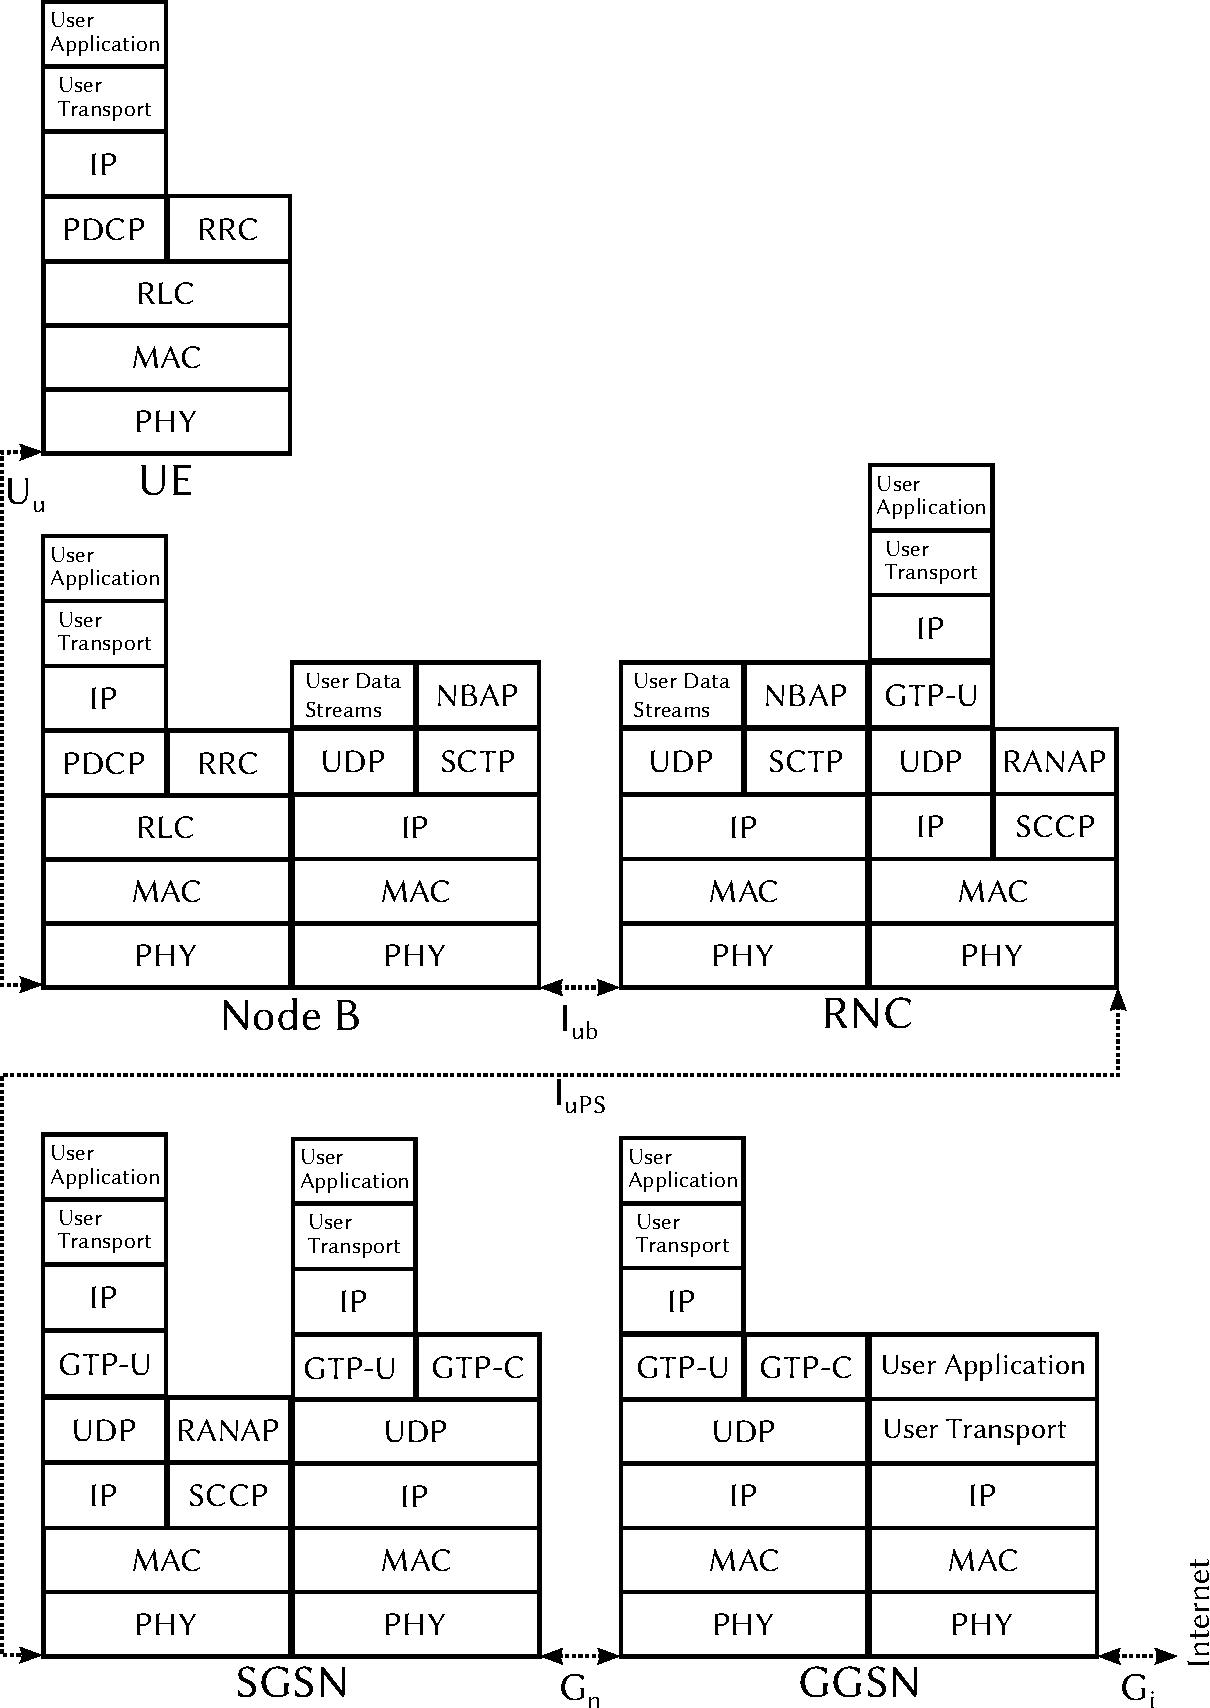
\includegraphics[width=0.9\textwidth]{images/umts-userpath-stack.pdf}
 	\caption{Simplified control plane and user plane \gls{IP}-based protocol stacks on the user traffic path through the mobile network.}
\label{c4:fig:protocolstacks}
\end{figure}

Figure~\ref{c4:fig:protocolstacks} overviews the complete protocol stack on the path of the user traffic through the whole network from the \gls{UE} to an external network.


%%
\subsection{Core Network Concepts}

Most of the discussed upcoming research deals with the core network. Therefore, this next sections will explain in detail the concepts behind the \gls{3G} core network control plane at the \gls{gtp} protocol family.

As stated, there is a strict separation between control instances and instances that carry the actual user traffic. Looking at the control plane side of things, management is conducted in a completely stateful way. Nodes keep track of every \gls{UE} they are managing and need to locally store any state information they might need for management purposes. Of particular interest is the state revolving around the \textit{\gls{PDP} Context}. For each open data connection a device has, both the \gls{GGSN} and \gls{SGSN} must keep such a \gls{PDP} Context, which identifies the connection as well as the device belonging to it.

Additionally, a number of state machines are maintained. Transitions between states in them then trigger a signaling message to specific neighbors. Any one of these signaling interactions belongs to one or more larger control plane procedures. Most of the procedures that happen inside the core network \gls{PS} domain or affect it are defined in \gls{TS}~24.008~\cite{3gpp.24.008} and \gls{TS}~23.060\cite{3gpp.23.060}.

\begin{figure}[htbp]
	\centering
	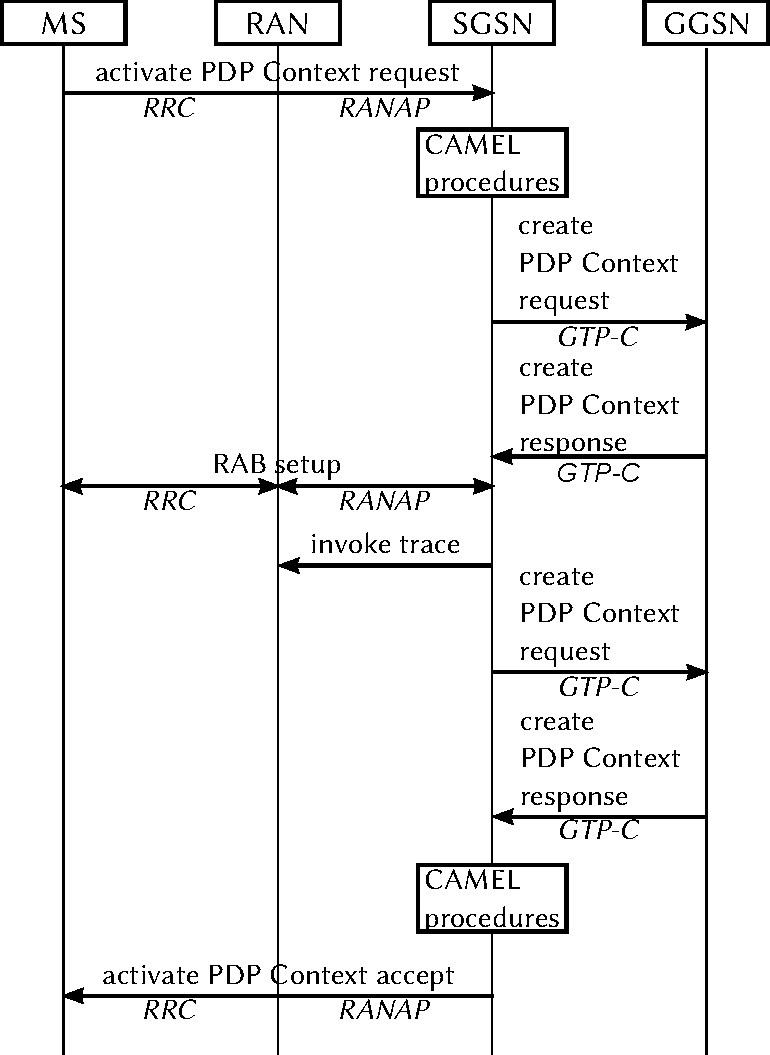
\includegraphics[width=0.7\textwidth]{images/pdp-context-activation-procedure.pdf}
	\caption{\gls{PDP} Context activation procedure signaling interaction diagram for \gls{UMTS}, including involved signaling protocols.}
\label{c4:fig:pdpcontextactivationinteraction}
\end{figure}

A very simple example is demonstrated in Figure~\ref{c4:fig:pdpcontextactivationinteraction}. Initiated by the \gls{UE}'s session management state machine a data connection to the device is requested to be set up, triggering signaling with various protocols throughout the network. Additional secondary \gls{CAMEL} procedures, defined in \cite{3gpp.23.078}, are also triggered and conducted.

The general motif of control in \gls{3G} networks is rather different to that of the typical \gls{TCP}/\gls{IP} Internet stack. Whereas plain \gls{IP} stacks rely on the end-to-end principle and put most of the control inside the devices at the edge, in \gls{3G} control procedures are spread across the network. Coordinating this requires the discussed control plane and all of the explicit signaling interactions. This results in a rather high complexity but also gives the opportunity to investigate these mechanisms and implications the structures have on the performance.


%%
\subsection{Tunneling Concept: Bearers and \texorpdfstring{\acrshort{PDP}}{PDP} Contexts}

To enact the aforementioned user and control plane separation, a custom tunneling concept is used. Beginning at the \gls{UE}, the actual user \gls{IP} stack is never directly carried over the link's layer 1 and 2 protocols but always further encapsulated into so called \textit{bearer}. The specifications distinguish between the \textit{radio bearer} on the air interface, the \gls{RAB} denominates the path between the \gls{UE} and the \gls{CN}, where it is called \gls{CN} bearer.

Technically, different protocols with tunneling capability are used on each link. \gls{PDCP} is used on the radio link, \gls{GTP-U} is employed between the \gls{RAN} and the \gls{CN} and in the core between \gls{SGSN} and \gls{GGSN}. Closely related to the core network bearer are a number of information records stored and maintained at the two core nodes, the aforementioned \gls{PDP} Context. For every active bearer a context is stored containing identification and management information about it. Amongst others this includes device identifiers, e.g., \gls{IMSI} and \gls{IMEI}, tunnel identifiers (\gls{TEID}), and information about the intended public network (the \gls{APN}) , charging, and \gls{QoS} \cite[Section~13]{3gpp.23.060}.

Commonly, any device with an active data connection has at least one bearer and an associated \gls{PDP} Context, the \textit{default bearer}. In terms of \gls{QoS} this represents a best effort tunnel carrying all user traffic, that is not further differentiated. Additionally, the device can request a number of secondary tunnels, i.e., \textit{dedicated bearers}, with certain \gls{QoS} guarantees. Traffic matching a specified \gls{TFT} will then be carried over this dedicated bearer. However, this concept is scarcely used in \gls{3G} networks. All in all, one \gls{UE} can be associated with up to eleven bearers, one default bearer and additional dedicated bearers.


%%
\subsection{\texorpdfstring{\acrshort{gtp}}{GTP} and \texorpdfstring{\acrshort{gtp}}{GTP}-based Core Network Signaling}
\label{c4:sec:gtp}

A large part of core network communication is conducted by \gls{gtp}. In \gls{3G} networks version 1 of the protocol is used and defined in \gls{TS}~29.060~\cite{3gpp.29.060} and \gls{TS}~29.281~\cite{3gpp.29.281}.\footnote{For a more concise description of the protocol, one should actually read the \gls{gtp} implementation in the community \gls{FOSS} project OpenGGSN at \url{https://github.com/osmobuntu/openggsn}.} For \gls{EPC} some changes were made to \gls{gtp} bringing it to version 2, which is specified in \gls{TS}~29.274~\cite{3gpp.29.274}. The latter will not be further discussed as all presented evaluations will have a \gls{3G} network as basis.

\gls{gtp} is mainly used on the Gn interface that connects the two main \gls{GPRS} nodes, the \gls{GGSN} and \gls{SGSN}. Its functionality is split up between a user plane and a control plane part, named respectively \gls{GTP-U} and \gls{GTP-C}. \gls{gtp} can best be described as an application layer signaling protocol and is intended to be transported by \gls{UDP}.

\begin{figure}[htb]
	\begin{tabu}{X[1]|X[1]|X[1]|X[1]|X[1]|X[1]|X[1]|X[1]|X[1]|}
	\multicolumn{1}{c}{} & \multicolumn{8}{c}{\textbf{Bits}} \\
	\textbf{Octets} & \textbf{8} & \textbf{7} & \textbf{6} & \textbf{5} & \textbf{4} & \textbf{3} & \textbf{2} & \textbf{1} \\ 
	\cline{2-9} \textbf{1} & \multicolumn{3}{c|}{Version}  & 1 & 0 & E & S & PN \\ 
	\cline{2-9} \textbf{2} & \multicolumn{8}{c|}{Message Type}  \\ 
	\cline{2-9} \textbf{3} & \multicolumn{8}{c|}{\multirow{2}{*}{Length}}  \\ 
				\textbf{4} & \multicolumn{8}{c|}{}  \\ 
	\cline{2-9} \textbf{5} & \multicolumn{8}{c|}{\multirow{4}{*}{Tunnel Endpoint Identifier}} \\ 
				\textbf{6} & \multicolumn{8}{c|}{} \\ 
				\textbf{7} & \multicolumn{8}{c|}{} \\ 
				\textbf{8} & \multicolumn{8}{c|}{} \\ 
	\cline{2-9} \textbf{9} & \multicolumn{8}{c|}{\multirow{2}{*}{Sequence Number}} \\
				\textbf{10} & \multicolumn{8}{c|}{} \\
	\cline{2-9}	\textbf{11} & \multicolumn{8}{c|}{N-PDU} \\
	\cline{2-9} \textbf{12} & \multicolumn{8}{c|}{Next Extension Header Type} \\
	\cline{2-9}
	\end{tabu} 
	\caption{General \SI{12}{\byte} \gls{gtp} header format.}
\label{c4:fig:gtpheader}
\end{figure}

Conceptually, \gls{gtp} is structured through a base packet header, a number of extension headers and a message body consisting of a series of \gls{IE}. The base header is depicted in Figure~\ref{c4:fig:gtpheader} and has a total length of \SI{12}{\byte}. Essential to the header are the \gls{TEID} to identify the corresponding user plane tunnel and the \SI{8}{\bit} message type field. Each of the message types corresponds to a specific signaling interaction from the overarching control plane procedures. The procedures that \gls{gtp} concerns itself with on the Gn path belong either to path management, tunnel management, or mobility management. Messages also usually come in request and response pairs which must be sent from the receiving node back to the original requester.

Each messages is defined as a specific set of \glspl{IE}, each of which is either mandatory, conditional to some external factor, or optional. These \gls{IE}, depending on the type either of fixed or variable length, convey the actual state to be signaled and always relate to a specific \gls{UE} and tunnel, for example the device's \gls{IMSI} or the configured \gls{APN}.

\begin{table}[htbp]
\caption{All \gls{IE} in a Create \gls{PDP} Context request and size thereof for \gls{IPv4} network and user traffic only. The denoted sizes exclude the first message type byte.}
\label{c4:tab:createrequestelements}
	\begin{tabu} to 0.49\textwidth{X[2.5]X[1.2]X[0.7]}
		\toprule
		\textbf{\gls{IE}} & \textbf{Presence} & \textbf{Size}\\
		\midrule
		\gls{IMSI} & cond. & \SI{8}{\byte} \\ 
		\acrshort{RAI} & opt. & \SI{6}{\byte} \\
		Recovery & opt. & \SI{1}{\byte} \\
		Selection mode	& cond. & \SI{1}{\byte} \\
		\gls{TEID} Data I & mand. & \SI{4}{\byte} \\
		\gls{TEID} Control Plane & cond. & \SI{4}{\byte} \\
		\gls{NSAPI} & mand. & \SI{1}{\byte} \\
		Linked \gls{NSAPI} & cond. & \SI{1}{\byte} \\
		Charging Characteristics & cond. & \SI{2}{\byte} \\
		Trace Reference & opt. & \SI{2}{\byte} \\
		Trace Type & opt. & \SI{2}{\byte} \\
		End User Address & cond. & \SI{8}{\byte} \\
		\gls{APN} & cond. & max \SI{102}{\byte} \\ % APN format defined in 23.003 section 9
		\acrshort{PCO} & opt. & max \SI{255}{\byte} \\ % defined in 24.008 section 10.5.6.3
		\gls{SGSN} signaling address & mand.  & \SI{6}{\byte} \\ % defined in 23.003 section 5 (without address type and length fields)
		\gls{SGSN} user traffic address & mand. & \SI{6}{\byte} \\ % same as above
		\gls{MSISDN} & cond. & max \SI{17}{\byte} \\ % ITU-T E.164 msisdn format recommendation of max 15 chars
		\gls{QoS} Profile & mand. & max \SI{257}{\byte} \\
		\bottomrule
	\end{tabu}%
	\raisebox{0.95mm}{\begin{tabu} to 0.49\textwidth{X[2.5]X[1.2]X[0.7]}
		\toprule
		\textbf{\gls{IE}} & \textbf{Presence} & \textbf{Size} \\
		\midrule
		\gls{TFT} & cond. & max \SI{257}{\byte} \\ % defined in 24.008 section 10.5.6.12
		 Trigger Id & opt. & var. \\ % no definition found
		 \acrshort{OMC} Identity & opt. & var. \\ % maybe in MAP 29.002, however not further definition found
		 Common Flags & opt. & \SI{3}{\byte} \\
		 \gls{APN} Restriction & opt. & \SI{3}{\byte} \\
		 \gls{RAT} & opt. & \SI{3}{\byte} \\
		 User Location Information & opt. & \SI{10}{\byte} \\
		 \gls{MS} Time Zone & opt. & \SI{4}{\byte} \\
		 \gls{IMEI} (\acrshort{SV}) & cond. & \SI{10}{\byte} \\
		 \gls{CAMEL} Charging Information Container & opt. & var. \\
		 Additional Trace Info & opt. & \SI{11}{\byte} \\
		 Correlation-ID & opt. & \SI{3}{\byte} \\
		 Evolved Allocation Retention Priority I & opt. & \SI{3}{\byte} \\
		 Extended Common Flags & opt. & \SI{3}{\byte} \\ % might be more, but seems unused 
		 User \acrshort{CSG} Information & opt. & \SI{10}{\byte} \\
		 \gls{APN}-\acrshort{AMBR} & opt.  & \SI{11}{\byte} \\
		 Signaling Priority Indication & opt. & \SI{3}{\byte} \\ % might be more, but seems unused
		 Private Extension & opt. & var. \\
		 \bottomrule
	\end{tabu}}
	%\vfill
	%\null
\end{table}

Coming back to the described \gls{PDP} Context activation procedure, it contains both the \gls{gtp} message \textit{Create \gls{PDP} Context request} as well as the \textit{response} twice. Such a Create request consists of the 36 \gls{IE} depicted in Table~\ref{c4:tab:createrequestelements}. Neglecting the elements which have no predefined upper length bound (besides the default \SI{16}{\bit} \gls{IE} length field) and assuming a maximum length for the other variable elements this results in a message size of \SI{1059}{\byte}. The complexity of the other message types is comparable.

One of the conducted investigations is that of the core network load, which will be defined and discussed later in detail. \gls{gtp} messages could play an interesting role here as they may directly or indirectly contribute to this load or at least be an indicator of load existing otherwise. Load could be caused by the generated network traffic as well as the assembly, processing, and storage of the involved state in form of the \gls{IE}.

The following sections detail the three \gls{gtp} tunnel management message pairs involved in the maintenance of \gls{PDP} Contexts. These are the \textit{Create, Update,} and \textit{Delete \gls{PDP} Context requests} and \textit{responses}. They represent the basis for the core network investigations.


%%
\subsubsection{Create \gls{PDP} Context Message}

This message type is part of procedures that enable the \gls{PS} data connection and the \gls{gtp} tunnel for a mobile device. These are the \textbf{\gls{PDP} Context activation procedure} (already depicted in Figure~\ref{c4:fig:pdpcontextactivationinteraction}) and the \textbf{Secondary \gls{PDP} Context activation} for additional \gls{gtp} tunnels to the device with specific \gls{QoS} levels set. They are triggered by the mobile device through \gls{RRC}/\gls{RANAP} signaling during or following a \gls{GPRS} attach procedure.

When a \gls{GGSN} receives a create request from an \gls{SGSN}, it has to allocate the necessary resources for a \gls{PDP} Context. Depending on the outcome, a response is sent back, indicating the success or failure of the operation. Typical failures include failed user authentication, a lack of resource, or unrecoverable system failures and malformed or corrupted request.


%%
\subsubsection{Delete \gls{PDP} Context Message}

Similar to to Create Context messages, a \textbf{Delete \gls{PDP} Context request} and \textbf{response} always coincides with the termination of a \gls{gtp} tunnel and the removal of the associated \gls{PDP} Context. Together, these mark the beginning and the end of every user traffic tunnel, making them very interesting in determining tunnel properties and perfect candidates to indirectly identify tunnel durations in a core network investigation.

Deletes are either created through explicit \gls{PDP} Context deactivation procedures or play a part in \gls{GPRS} attach and detach procedures. Contrary to creates, they can be initiated from the \gls{MS} as well as from a core network node, depending on the kind of procedure.


%%
\subsubsection{Update \gls{PDP} Context Messages}

Several procedures also emit \textbf{Update \gls{PDP} Context requests} and \textbf{responses}, usually in relation to some aspect of the tunnel or the device changing. Possible causes for an \textit{Update Context request} are:

\begin{itemize}
	\item The mobile devices moves between \glspl{SGSN}, causing a \textbf{\gls{GPRS} inter-\gls{SGSN} Routing Area Update} procedure.
	\item Parameters belonging to the context such as the assigned \gls{QoS} are altered using the t\textit{\gls{PDP} Context Modification} procedure.
	\item As part of \textbf{Context redistribution and load balancing} procedures.
	\item The \gls{MS} switches between \gls{UMTS} and \gls{GPRS} access technologies, causing a \textit{Inter-system intra-\gls{SGSN} Update} procedure. Note that the same tunnel can be used regardless of the radio technology.
	\item As part of a direct \gls{RNC} to \gls{GGSN} \gls{GTP-U} tunnel activation procedure, thereby circumventing the \gls{SGSN}. Or, finally, 
	\item to activate secondary \gls{PDP} Contexts using the \textbf{Secondary PDP Context Activation} as previously described. 
\end{itemize}

However, the appearance of update message signaling in some of these procedures is conditional or even just optional. This often depends on the specific implementation and is not known without in-depth knowledge of it. An exception to this are mobility management procedures where updates are mandatory.

By observing update messages one could capture most forms of mobility happening in the network, and get a good picture of potential correlation between mobility and tunneling characteristics. 
By distinguishing portions of tunnels which were associated with a \gls{UMTS} \gls{RAB} from \gls{2G} radio access through the related update message, one could also study any influence of the access technology on the core.

Nowadays \gls{GSM}/\gls{GPRS} is either used in older models or feature phones or in mobile scenarios in rural areas where \gls{GSM} still is prevalent due to its usage of lower frequency bands and thus wider ranger. Both could indicate that the data session will be rather short because of device limited device capabilities or low throughput rates of \gls{GPRS}.


%%
\subsection{\texorpdfstring{\acrshort{gtp}}{GTP} Influencing State Machines}

To understand the occurrence of these signaling procedures one should look at the state machines that govern these. Involved in the tunnel management aspects are three distinct \gls{FSM}, namely the \gls{MM} and \gls{RRC} state machines and the actual \gls{PDP} state model. The \gls{MM} and \gls{RRC} describe the current state of the mobile device and its radio and data connection. They are both maintained at the \gls{MS} and mirrored at the\gls{SGSN}.

\begin{figure}[htb]
	\centering
	\begin{subfigure}[b]{0.60\textwidth}
		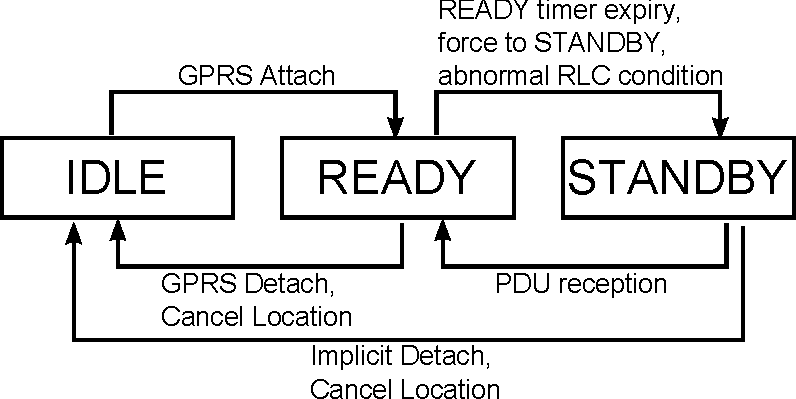
\includegraphics[width=\textwidth]{images/mm-2g-state-model.pdf}
		\caption{State machine for \gls{2G} radio access.}
		\label{c4:fig:2g-mmstatemodel}
	\end{subfigure}%

	\begin{subfigure}[b]{0.70\textwidth}
		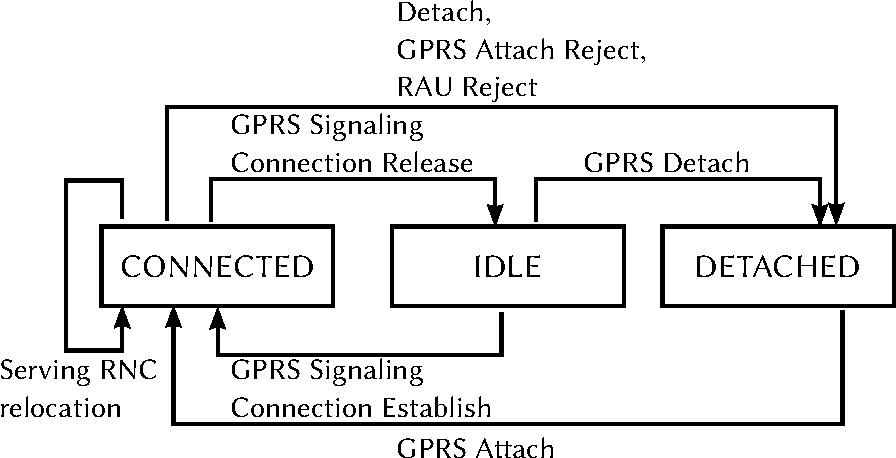
\includegraphics[width=\textwidth]{images/mm-3g-state-model.pdf}
		\caption{State machine for \gls{3G} radio access.}
		\label{c4:fig:3g-mmstatemodel}
	\end{subfigure}%
	\caption{\gls{SGSN} \gls{MM} state models and machines as defined in \cite[Section~6.1]{3gpp.23.060}.}
\label{c4:fig:mmstatemodel}
\end{figure}

The \gls{MM} model, defined in \cite[Section~6.1]{3gpp.23.060}, describes the general state of the data connection. State switches occur either based on an idle timer or when new packets arrive for the mobile device. The specific model depends on the currently used \gls{RAT} with only slight differences between \gls{GSM} (Figure~\ref{c4:fig:2g-mmstatemodel}) and \gls{UMTS} (Figure~\ref{c4:fig:3g-mmstatemodel}) access. The \gls{LTE} related model brings larger changes but is omitted here, as it will not be relevant for the investigation. With the transition to and from the \textbf{IDLE} state in the \gls{2G} model (or \textbf{DETACHED} in \gls{3G}) \textbf{GPRS Attach/Detach} procedures are triggered, also resulting in the transmission of \gls{PDP} Create and Delete Context messages. Likewise, other state transition procedures indicate mobility and location changes, which usually include update messages.

\begin{figure}[htb] 
	\centering
	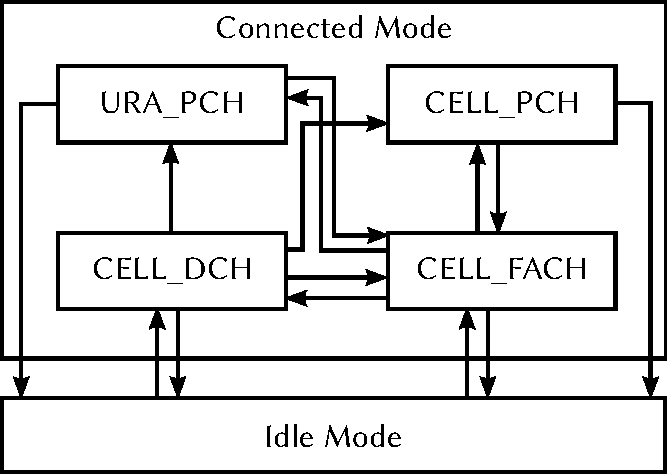
\includegraphics[width=0.6\textwidth]{images/rrc-state-model.pdf}
	\caption{\gls{RRC} State Model as per \cite[Section~7.1]{3gpp.25.331}.}
	\label{c4:fig:rrcstatemodel}
\end{figure}

 The \gls{RRC} state machine given in \gls{TS}~25.331~\cite[Section~7.1]{3gpp.25.331} and depicted in Figure~\ref{c4:fig:rrcstatemodel} governs the usage of radio channels and therefore power states of the \gls{MS}. State changes happen depending on user and radio activity and inactivity determined by timers. Only in the \gls{CELLDCH} state is the \gls{MS} assigned a dedicated channel for its data connection and can transmit at full bidirectionally. But this consumes the most device power and radio resources, both of which are scarce. The goal of the state machine is to minimize resource usage with intermediary states --- \gls{CELLFACH}, \gls{URAPCH}, and \gls{CELLPCH}, and  --- that successively require less power and radio channels, before completely turning of the \gls{RRC} connection by transitioning to the idle state. Coinciding with the \gls{RRC}, the \gls{CN} \gls{gtp} tunnel can also be released or needs to be reestablished. However, this is implementation specific and not precisely specified.

\begin{figure}[htb]
	\centering
	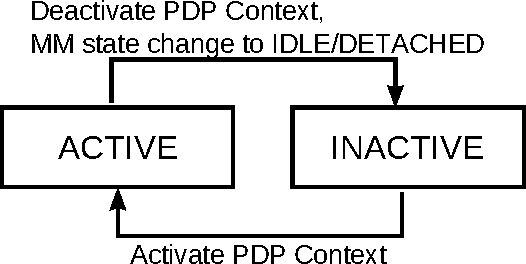
\includegraphics[width=0.5\textwidth]{images/pdp-state-model.pdf}
	\caption{\gls{PDP} State Model defined in \cite[Section~9]{3gpp.23.060}.}
\label{c4:fig:pdpstatemodel}
\end{figure}

The final state machine of relevancy is the \textbf{\gls{PDP} State Model} from \gls{TS}~23.060~\cite[Section~9]{3gpp.23.060} in Figure~\ref{c4:fig:pdpstatemodel}. It reflects the actual state of the \gls{PDP} context and associated tunnel and is synchronized with the \gls{MM} state machine.


%%
\subsection{Signaling Discussion}

This section on the basics of current mobile network architectures serves a critical purpose: In order to measure and evaluate network traffic one has to first understand its architecture and needs to grasp how certain traffic patterns can occur. Unfortunately, the \gls{3GPP} specifications do not make this task very easy. Typical \gls{IETF} protocols and architectures sadhere to the fundamental principles of protocol layering, function separation and end-to-end. One can read a single \gls{RFC} and understand its function and directly implement it independent of the knowledge of any other specification. This is not the case in a \gls{3G} network. Functions are often spread over several protocols or nodes, necessary details essential to an implementation are spread out over several specifications without direct reference or are even completely omitted. This circumstance makes it very hard to attribute certain observed phenomena to a specific feature in the specification.

These protocols are also very heavy in terms of state and signaling inside the network. This can be the cause of unintended and hard to predict load, which will be defined and discussed in Section~\ref{c4:sec:loaddefinition}. For now, some possibly load information in relation to the Create, Update and Delete \gls{PDP} Context Request and Reply message pairs can already be deduced. Measuring the time delta between corresponding Create and Delete events obviously results in the total duration a tunnel was established. Having shorter tunnels often also means having a greater number of tunnels and therefore a higher volume of signaling messages and an increase in processing and state-keeping efforts due to the signaling. 

Conversely, longer tunnel durations cause an increased overall memory footprint in the involved nodes to store the \gls{PDP} Contexts. Large numbers of update messages, especially combined with frequent \gls{RAT} switches, are usually an indicator for highly mobile devices switching their routing area. The time between a request and its corresponding response could also be an indicator for the amount of processing involved for this message as well as the current general processing load at the \gls{GGSN}. Most of the actions in the network as well as in the mobile devices are reflected in the presented tunnel management messaging. Therefore, taking a look at the dynamics of this control aspect in real networks gives valuable insights on the influence of many of the networks' aspects.





%This section starts with a primer on cellular data network basics, and then moves on to describe relevant details of \gls{gtp}, the tunneling protocol under investigation.


% calculation: 36 element lengths + 36 * 1 Byte IE type fields + 11 byte header with no extensions
% 1012 + 36 + 11 = 1059B



% http://3gppinterview.blogspot.co.at/p/why-is-cellfach-and-cellpch-not.html <- this may be easier to understand


% \subsubsection{Information Elements Wire Format}

% \paragraph{IMSI}

% \begin{table}[htb]
% 	\caption{IMSI Information Element Format.}
% 	\label{c4:tbl:imsiieformat}
% 	\begin{tabu}{X[c]|X|X|X|X|X|X|X|X|}
% 	\multicolumn{1}{c}{} & \multicolumn{8}{c}{\textbf{Bits}} \\
% 	\cline{2-9} \textbf{Octets} & 8 & 7 & 6 & 5 & 4 & 3 & 2 & 1 \\ 
% 	\cline{2-9} 1 & \multicolumn{8}{c|}{Type = 1 (decimal)} \\ 
% 	\cline{2-9} 2 to 3 & \multicolumn{8}{c|}{Length = n}  \\ 
% 	\cline{2-9} 4 & \multicolumn{4}{c|}{Spare} & \multicolumn{4}{c|}{Instance} \\ 
% 	\cline{2-9} 5 & \multicolumn{4}{c|}{Number digit 2} & \multicolumn{4}{c|}{Number digit 1} \\ 
% 	\cline{2-9} 6 & \multicolumn{4}{c|}{Number digit 4} & \multicolumn{4}{c|}{Number digit 3} \\ 
% 	\cline{2-9} ... & \multicolumn{4}{c|}{...} & \multicolumn{4}{c|}{...} \\ 
% 	\cline{2-9} n+4 & \multicolumn{4}{c|}{Number digit m} & \multicolumn{4}{c|}{Number digit m-1} \\ 
% 	\cline{2-9}
% 	\end{tabu}
% \end{table}

% Decimals coded as TBCD; if odd number fill last nibble with 1; max digits is 15.\\
% Max IE size 12 Byte.

% \paragraph{APN}

% \begin{table}[htb]
% 	\caption{APN Information Element Format.}
% 	\label{c4:tbl:apnieformat}
% 	\begin{tabu}{X[c]|X|X|X|X|X|X|X|X|}
% 	\multicolumn{1}{c}{} & \multicolumn{8}{c}{\textbf{Bits}} \\
% 	\cline{2-9} \textbf{Octets} & 8 & 7 & 6 & 5 & 4 & 3 & 2 & 1 \\ 
% 	\cline{2-9} 1 & \multicolumn{8}{c|}{Type = 71 (decimal)} \\ 
% 	\cline{2-9} 2 to 3 & \multicolumn{8}{c|}{Length = n}  \\ 
% 	\cline{2-9} 4 & \multicolumn{4}{c|}{Spare} & \multicolumn{4}{c|}{Instance} \\ 
% 	\cline{2-9} 5 to (n+4) & \multicolumn{8}{c|}{Access Point Name} \\ 
% 	\cline{2-9}
% 	\end{tabu} 
% \end{table}

% Full APN name including APN Network Identifier and APN Operator Identifier.
% Network Identifier: max length 63 bytes.
% Operator Identifier: mnc<3digits>.mcc<3digits>.gprs; 16 bytes (18 incl dots).
% (Ex: ggsn-cluster-A.provinceB.mnc012.mcc345.gprs)

% Max total $4+63+16=83$

% \paragraph{AMBR}

% \begin{table}[htb]
% 	\caption{APN Information Element Format.}
% 	\label{c4:tbl:abmrieformat}
% 	\begin{tabu}{X[c]|X|X|X|X|X|X|X|X|}
% 	\multicolumn{1}{c}{} & \multicolumn{8}{c}{\textbf{Bits}} \\
% 	\cline{2-9} \textbf{Octets} & 8 & 7 & 6 & 5 & 4 & 3 & 2 & 1 \\ 
% 	\cline{2-9} 1 & \multicolumn{8}{c|}{Type = 72 (decimal)} \\ 
% 	\cline{2-9} 2 to 3 & \multicolumn{8}{c|}{Length = n}  \\ 
% 	\cline{2-9} 4 & \multicolumn{4}{c|}{Spare} & \multicolumn{4}{c|}{Instance} \\ 
% 	\cline{2-9} 5 to 8 & \multicolumn{8}{c|}{APN-AMBR for uplink} \\ 
% 	\cline{2-9} 9 to 12 & \multicolumn{8}{c|}{APN-AMBR for downlink} \\ 
% 	\cline{2-9}
% 	\end{tabu} 
% \end{table}

% Total size 12 bytes.


% \paragraph{Recovery}

% \begin{table}[htb]
% 	\caption{Recovery Information Element Format.}
% 	\label{c4:tbl:recoveryieformat}
% 	\begin{tabu}{X[c]|X|X|X|X|X|X|X|X|}
% 	\multicolumn{1}{c}{} & \multicolumn{8}{c}{\textbf{Bits}} \\
% 	\cline{2-9} \textbf{Octets} & 8 & 7 & 6 & 5 & 4 & 3 & 2 & 1 \\ 
% 	\cline{2-9} 1 & \multicolumn{8}{c|}{Type = 3 (decimal)} \\ 
% 	\cline{2-9} 2 to 3 & \multicolumn{8}{c|}{Length = n}  \\ 
% 	\cline{2-9} 4 & \multicolumn{4}{c|}{Spare} & \multicolumn{4}{c|}{Instance} \\ 
% 	\cline{2-9} 5 to (n+4) & \multicolumn{8}{c|}{Recovery (Restart Counter} \\ 
% 	\cline{2-9}
% 	\end{tabu} 
% \end{table}

% IN GTPv2 first release IE length is 5 bytes. May be longer in the future.


% \paragraph{MEI}

% \begin{table}[htb]
% 	\caption{MEI Information Element Format.}
% 	\label{c4:tbl:meiieformat}
% 	\begin{tabu}{X[c]|X|X|X|X|X|X|X|X|}
% 	\multicolumn{1}{c}{} & \multicolumn{8}{c}{\textbf{Bits}} \\
% 	\cline{2-9} \textbf{Octets} & 8 & 7 & 6 & 5 & 4 & 3 & 2 & 1 \\ 
% 	\cline{2-9} 1 & \multicolumn{8}{c|}{Type = 75 (decimal)} \\ 
% 	\cline{2-9} 2 to 3 & \multicolumn{8}{c|}{Length = n}  \\ 
% 	\cline{2-9} 4 & \multicolumn{4}{c|}{Spare} & \multicolumn{4}{c|}{Instance} \\ 
% 	\cline{2-9} 5 to (n+4) & \multicolumn{8}{c|}{Mobile Equipment (ME) Identity} \\ 
% 	\cline{2-9}
% 	\end{tabu}
% \end{table}

% 15 (IMEI) or 16 (IMEISV) BCD digits filled with 1 to full octet. Size is 12 bytes.

% \paragraph{MSISDN}

% \begin{table}[htb]
% 	\caption{MSISDN Information Element Format.}
% 	\label{c4:tbl:msisdnieformat}
% 	\begin{tabu}{X[c]|X|X|X|X|X|X|X|X|}
% 	\multicolumn{1}{c}{} & \multicolumn{8}{c}{\textbf{Bits}} \\
% 	\cline{2-9} \textbf{Octets} & 8 & 7 & 6 & 5 & 4 & 3 & 2 & 1 \\ 
% 	\cline{2-9} 1 & \multicolumn{8}{c|}{Type = 76 (decimal)} \\ 
% 	\cline{2-9} 2 to 3 & \multicolumn{8}{c|}{Length = n}  \\ 
% 	\cline{2-9} 4 & \multicolumn{4}{c|}{Spare} & \multicolumn{4}{c|}{Instance} \\ 
% 	\cline{2-9} 5 & \multicolumn{4}{c|}{Number digit 2} & \multicolumn{4}{c|}{Number digit 1} \\ 
% 	\cline{2-9} 6 & \multicolumn{4}{c|}{Number digit 4} & \multicolumn{4}{c|}{Number digit 3} \\ 
% 	\cline{2-9} ... & \multicolumn{4}{c|}{...} & \multicolumn{4}{c|}{...} \\ 
% 	\cline{2-9} n+4 & \multicolumn{4}{c|}{Number digit m} & \multicolumn{4}{c|}{Number digit m-1} \\ 
% 	\cline{2-9}
% 	\end{tabu}
% \end{table}

% MSISDN limited to 15 digits. Max total size 12 bytes.


% \paragraph{Indication}

% \begin{table}[htb]
% 	\caption{Indication Information Element Format.}
% 	\label{c4:tbl:indicationieformat}
% 	\begin{tabu}{X[c]|X|X|X|X|X|X|X|X|}
% 	\multicolumn{1}{c}{} & \multicolumn{8}{c}{\textbf{Bits}} \\
% 	\cline{2-9} \textbf{Octets} & 8 & 7 & 6 & 5 & 4 & 3 & 2 & 1 \\ 
% 	\cline{2-9} 1 & \multicolumn{8}{c|}{Type = 77 (decimal)} \\ 
% 	\cline{2-9} 2 to 3 & \multicolumn{8}{c|}{Length = n}  \\ 
% 	\cline{2-9} 4 & \multicolumn{4}{c|}{Spare} & \multicolumn{4}{c|}{Instance} \\ 
% 	\cline{2-9} 5 & DAF & DTF & HI & DFI & OI & ISRSI & ISRAI & SGWCI \\ 
% 	\cline{2-9} 6 & Spare & UIMSI & CFSI & CRSI & P & PT & SI & MSV \\ 
% 	\cline{2-9} 7 to (n+4) & \multicolumn{8}{c|}{These octet(s) is/are present only if explicitly specified} \\ 
% 	\cline{2-9}
% 	\end{tabu}
% \end{table}

% Size is 7 bytes.

% \paragraph{PCO}


% \begin{table}[htb]
% 	\caption{PCO Information Element Format.}
% 	\label{c4:tbl:pcoieformat}
% 	\begin{tabu}{X[c]|X|X|X|X|X|X|X|X|}
% 	\multicolumn{1}{c}{} & \multicolumn{8}{c}{\textbf{Bits}} \\
% 	\cline{2-9} \textbf{Octets} & 8 & 7 & 6 & 5 & 4 & 3 & 2 & 1 \\ 
% 	\cline{2-9} 1 & \multicolumn{8}{c|}{Type = 78 (decimal)} \\ 
% 	\cline{2-9} 2 to 3 & \multicolumn{8}{c|}{Length = n}  \\ 
% 	\cline{2-9} 4 & \multicolumn{4}{c|}{Spare} & \multicolumn{4}{c|}{Instance} \\ 
% 	\cline{2-9} 5 to (n+4) & \multicolumn{8}{c|}{Protocol Configuration Options} \\
% 	\cline{2-9}
% 	\end{tabu}
% \end{table}

% Minimum length 4+3-3, maximum length 4+253-3; average?


% \paragraph{PAA}

% \begin{table}[htb]
% 	\caption{PAA Information Element Format.}
% 	\label{c4:tbl:paaieformat}
% 	\begin{tabu}{X[c]|X|X|X|X|X|X|X|X|}
% 	\multicolumn{1}{c}{} & \multicolumn{8}{c}{\textbf{Bits}} \\
% 	\cline{2-9} \textbf{Octets} & 8 & 7 & 6 & 5 & 4 & 3 & 2 & 1 \\ 
% 	\cline{2-9} 1 & \multicolumn{8}{c|}{Type = 79 (decimal)} \\ 
% 	\cline{2-9} 2 to 3 & \multicolumn{8}{c|}{Length = n}  \\ 
% 	\cline{2-9} 4 & \multicolumn{4}{c|}{Spare} & \multicolumn{4}{c|}{Instance} \\ 
% 	\cline{2-9} 5 & \multicolumn{5}{c|}{Spare} & \multicolumn{3}{c|}{PDN Type} \\
% 	\cline{2-9} 6 to (n+4) & \multicolumn{8}{c|}{PDN Adress and Prefix} \\
% 	\cline{2-9}
% 	\end{tabu} 
% \end{table}

% Either 9 (IPv4), 22 (IPv6), or 26 (IPv4v6).


% \paragraph{RAT Type}


% \begin{table}[htb]
% 	\caption{RAT Information Element Format.}
% 	\label{c4:tbl:ratieformat}
% 	\begin{tabu}{X[c]|X|X|X|X|X|X|X|X|}
% 	\multicolumn{1}{c}{} & \multicolumn{8}{c}{\textbf{Bits}} \\
% 	\cline{2-9} \textbf{Octets} & 8 & 7 & 6 & 5 & 4 & 3 & 2 & 1 \\ 
% 	\cline{2-9} 1 & \multicolumn{8}{c|}{Type = 82 (decimal)} \\ 
% 	\cline{2-9} 2 to 3 & \multicolumn{8}{c|}{Length = n}  \\ 
% 	\cline{2-9} 4 & \multicolumn{4}{c|}{Spare} & \multicolumn{4}{c|}{Instance} \\ 
% 	\cline{2-9} 5 & \multicolumn{8}{c|}{RAT Type} \\
% 	\cline{2-9} 6 to (n+4) & \multicolumn{8}{c|}{These octet(s) is/are present only if explicitly specified} \\
% 	\cline{2-9}
% 	\end{tabu} 
% \end{table}

% Maximum length 5 to ?.

% \paragraph{Serving Network}

% \begin{table}[htb]
% 	\caption{Serving Network Information Element Format.}
% 	\label{c4:tbl:servingnetieformat}
% 	\begin{tabu}{X[c]|X|X|X|X|X|X|X|X|}
% 	\multicolumn{1}{c}{} & \multicolumn{8}{c}{\textbf{Bits}} \\
% 	\cline{2-9} \textbf{Octets} & 8 & 7 & 6 & 5 & 4 & 3 & 2 & 1 \\ 
% 	\cline{2-9} 1 & \multicolumn{8}{c|}{Type = 83 (decimal)} \\ 
% 	\cline{2-9} 2 to 3 & \multicolumn{8}{c|}{Length = n}  \\ 
% 	\cline{2-9} 4 & \multicolumn{4}{c|}{Spare} & \multicolumn{4}{c|}{Instance} \\ 
% 	\cline{2-9} 5 & \multicolumn{4}{c|}{MCC digit 2} & \multicolumn{4}{c|}{MCC digit 1} \\ 
% 	\cline{2-9} 6 & \multicolumn{4}{c|}{MNC digit 3} & \multicolumn{4}{c|}{MCC digit 3} \\ 
% 	\cline{2-9} 7 & \multicolumn{4}{c|}{MNC digit 2} & \multicolumn{4}{c|}{MNC digit 1} \\ 
% 	\cline{2-9} 8 to (n+4) & \multicolumn{8}{c|}{These octet(s) is/are present only if explicitly specified} \\
% 	\cline{2-9}
% 	\end{tabu}
% \end{table} 

% Maximum length 7 to ?.


% \paragraph{User Location Information}

% \begin{table}[htb]
% 	\caption{User Location Information Element Format.}
% 	\label{c4:tbl:userlocieformat}
% 	\begin{tabu}{X[c]|X|X|X|X|X|X|X|X|}
% 	\multicolumn{1}{c}{} & \multicolumn{8}{c}{\textbf{Bits}} \\
% 	\cline{2-9} \textbf{Octets} & 8 & 7 & 6 & 5 & 4 & 3 & 2 & 1 \\ 
% 	\cline{2-9} 1 & \multicolumn{8}{c|}{Type = 86 (decimal)} \\ 
% 	\cline{2-9} 2 to 3 & \multicolumn{8}{c|}{Length = n}  \\ 
% 	\cline{2-9} 4 & \multicolumn{4}{c|}{Spare} & \multicolumn{4}{c|}{Instance} \\ 
% 	\cline{2-9} 5 & \multicolumn{3}{c|}{Spare} & ECGI & TAI & RAI & SAI & CGI \\ 
% 	\cline{2-9} a to a+6 & \multicolumn{8}{c|}{CGI} \\ 
% 	\cline{2-9} 7 & \multicolumn{8}{c|}{SAI} \\ 
% 	\cline{2-9} 7 & \multicolumn{8}{c|}{RAI} \\ 
% 	\cline{2-9} 7 & \multicolumn{8}{c|}{TAI} \\ 
% 	\cline{2-9} 7 & \multicolumn{8}{c|}{ECGI} \\ 
% 	\cline{2-9} 8 to (n+4) & \multicolumn{8}{c|}{These octet(s) is/are present only if explicitly specified} \\
% 	\cline{2-9}
% 	\end{tabu} 
% \end{table}



% Information Elements Table for PDP Context Activation Case only for GTPv2 (LTE)
% \begin{longtabu} to\linewidth{| X[2,l] | X[2,c] | X[l] | X[4] |}
% \hline
% Information Element 						& IE Type 					& Max Wire Size (Bytes)	& Comment \\ \hline
% \gls{IMSI} 										& IMSI 						& 12					& \\ \hline
% \gls{MSISDN} 										& MSISDN					& 12					& On S11 Interface if provided by HSS; In case of UE requested connectivity if MME has it stored. \\ \hline
% MEI Identity 								& MEI 						& 12					& If available at MME. \\ \hline
% User Location Information 					& ULI						& 						& E-UTRAN initial attach \&  UE requested connectivity only; included by S-GW if received from MME via S5/S8; included on S4 and S5/S8 for PDP context activation, either CGI, SAI, or RAI. \\ \hline
% Serving Network								& Serving Network			& 						& Initial E-UTRAN attach, context activation and UE requested connectivity \\ \hline
% \gls{RAT} Type									& RAT Type					& 5						& \\ \hline
% Indication Flags							& Indication				& 6						& Flags: S5/S8 Protocol Type; Dual Address Bearer Flag; Handover Indication; Direct Tunnel Flag; Piggybacking Supported; Change Reporting Support Indication \\ \hline
% Sender F-TEID for Control Plane				& F-TEID					& 						& \\ \hline
% P-G S5/S8 Address for Control Plane or PMIP	& F-TEID					& 						& On S11/S4 interfaces; 0 if initial attach, context activation or PDN connectivity \\ \hline
% Access Point Name							& APN						& 83					& \\ \hline
% Selection Mode								& Selection Mode			& 						& Indicate whether subscribed or non-subscribed, chosen by MME, was selected \\ \hline
% PDN Type									& PDN Type					& 						& IPv4, IPv6 or IPv4v6. \\ \hline
% PDN Address Allocation						& PAA						& 26					& Set to static IP address; else (dynamic) to 0.0.0.0 or IPv6 Prefix Length 0. \\ \hline
% Maximum APN Restriction						& APN Restriction			& 						& Set to most stringent restriction of any active bearer. \\ \hline
% Aggregate Maximum Bit Rate					& ABMR						& 12					& \\ \hline
% Protocol Configuration Options				& PCO						& 254					& Forwarded from UE to P-GW via S-GW via MME. \\ \hline
% Bearer Contexts to be created				& Bearer Context			& 						& present multiple times to represent list of bearers \\ \hline
% Trace Information							& Trace Information 		& 						& If S-GW / P-GW is activated. \\ \hline
% Recovery									& Recovery					& 5						& If peer node contacted for the first time. \\ \hline
% MME-FQ-CSID									& FQ-CSID					& 						& Included by MME on S11 \\ \hline
% SGW-FQ-CSID									& FQ-CSID					& 						& Included by SGW on S5/S8 \\ \hline
% UE Time Zone								& UE Time Zone 				& 						& Can be included by MME on S11; forwarded to P-GW via S-GW \\ \hline
% User CSG Information						& UCI						& 						& If \gls{UE} accessed via CSG cell or hybrid cell \\ \hline
% Charging Characteristics					& Charging Characteristics	&						& \\ \hline
% Private Extensions							& Private Extensions		&						& \\ \hline
% \end{longtabu}





% \begin{figure}[htb]
% 	\centering
%  	\includegraphics[width=0.9\textwidth]{images/eNB-MME-layers.pdf}
%  	\caption{Control plane protocol stack at the S1-MME interface between eNodeB and MME.}
%  	\label{c4:fig:stack-enbmme}
% \end{figure}

% \begin{figure}[htb]
% 	 \centering
% 	 \includegraphics[width=0.9\textwidth]{images/SGSN-MME-layers.pdf}
% 	 \caption{Control plane protocol stack at the S3 interface between SGSN and MME.}
% 	 \label{c4:fig:stack-sgsnmme}
% \end{figure}

% \begin{figure}[htb]
% 	\centering
% 	\includegraphics[width=0.9\textwidth]{images/S-GW-P-GW-layers.pdf}
% 	\caption{Optional control plane protocol stack at the S5 interface between SGW and PGW.}
% 	\label{c4:fig:stack-sgwpgw}
% \end{figure}

% \begin{figure}[htb]
% 	\centering
% 	\includegraphics[width=0.9\textwidth]{images/MME-S-GW-layers.pdf}
% 	\caption{Control plane protocol stack at the S11 interface between MME and SGW.}
% 	\label{c4:fig:stack-mmesgw}
% \end{figure}



%List of interfaces in the 3G/LTE PS network
%\begin{itemize}
%\item \textbf{Uu}: Interface between the mobile station (MS) and the fixed network part in Iu mode. The Uu interface is the Iu mode network interface for providing packet data services over the radio to the MS. The MT part of the MS is used to access the UMTS services through this interface.
%\item \textbf{Iub}: Interface between a NodeB and a RNC.
%\item \textbf{IuPS}: Interface between a RNC and a SGSN.
%\item \textbf{S1-U}: Interface between a eNodeB and a S-GW. User plane bearer tunneling.
% \item \textbf{S1-MME}: Interface between a eNodeB and a MME.
% \item \textbf{S3}: Interface between a SGSN and a MME. User/bearer information exchange for active/idle state 3g network access mobility.
% \item \textbf{S4}: Interface between a SGSN and a S-GW.	 2G user plane tunneling. GPRS mobility and control.
% \item \textbf{S5}: Interface between a S-GW and a P-GW within the same PLMN. User plane tunneling; S-GW relocation due to mobility.
% \item \textbf{S6a}: Interface between a MME and a HSS. Auth/auth data transfer to evolved system.
% \item \textbf{Gr/S6d}: Interface between a SGSN and a HSS. 
% \item \textbf{S8}: Interface between a S-GW and a P-GW in different PLMNs. Inter-PLMN variant to S5.
% \item \textbf{S9}: Interface between a PRCF and the packet data network. Data exchange to visited PCRF PLMN.
% \item \textbf{S11}: Interface between a S-GW and a MME.
% \item \textbf{S12}: UTRAN to S-GW reference point. Based on Iu-u/Gn-u. Direct Tunnel via GTP-U.
% \item \textbf{S13}: Interface between a MME and a EIR. UE identity check.
% \item \textbf{SGi}: The reference point between the EPC based PLMN and the packet data network. Same as Gi for 3gpp.

% \item \textbf{GC}: Interface between a HSS and a GGSN.
% \item \textbf{Gf}: Interface between a SGSN and a EIR.
% \item \textbf{Gi}: Reference point between Packet Domain and an external packet data network.
% \item \textbf{Gn}: Interface between two GSNs within the same PLMN.
% \item \textbf{Gp}: Interface between two GSNs in different PLMNs. The Gp interface allows support of Packet Domain network services across areas served by the co-operating PLMNs.
% \item \textbf{Gx}: Interface between a PCRF and a P-GW/GGSN. QoS policy and charging rules transfer.
% \item \textbf{Gxc}: Interface between a PCRF and a S-GW.

% \item \textbf{Rx}: Interface between a PRCF and the packet data network.
% \end{itemize}


%EMM Service request procedure
% \begin{figure}[htb]
% 	\centering
% 	\includegraphics[width=1.0\textwidth]{images/UE-service-request.pdf}
% 	\caption{EMM service request procedure sequence diagram.}
% 	\label{c4:fig:3gpp-ueservicereq}
% \end{figure}

% Annotations:
% 1. Encapsulated in RRC message.
% 2. Forwarded in S1-AP Initial UE Message.
% 3. Various security procedures.

%	25.401 \cite{3gpp.25.401} UTRAN overall description
%	25.931 \cite{3gpp.25.931} UTRAN functions, examples on signalling procedures
%	23.401 \cite{3gpp.23.401} \gls{E-UTRAN} procedures (LTE only)
%	24.007 \cite{3gpp.24.007} radio interface signaling % only Um interface in plain GSM/GPRS
%	36.300 \cite{3gpp.36.300} \gls{E-UTRAN} description (LTE only) 
%	36.414 \cite{3gpp.36.414} Evolved Universal Terrestrial Radio Access Network (E-UTRAN); S1 data transport (radio bearer)
%	22.060 \cite{3gpp.22.060} basic and short \gls{GPRS} service description; unchanged since Release 6 (2004)
%	23.060 \cite{3gpp.23.060} \gls{GPRS} description : \gls{GPRS} specific procedures, interfaces and nodes; mobility management; radio management; packet routing; operational aspects



	%23.402 \cite{3gpp.23.402} (LTE only) non-\gls{3GPP} accesses
	%24.301 \cite{3gpp.24.301} EPS Non-Access-Stratum protocol between UE and MME on Uu

% Relevant protocols and interfaces between nodes:
% \begin{itemize}
% 	\item \gls{gtp}, \gls{gtpv2}, GTP-u, GTP-c, \gls{SGSN} to \gls{GGSN} and others (specify!), on top of \gls{UDP}, GTPv1 will be described in detail in a separate section as it is at the core of the upcoming investigations.
% 	\item \gls{MAP} / \gls{SS7}: \gls{SGSN} - \gls{HLR}, \gls{GGSN} - \gls{HLR} and others; subscriber management and information exchange
% 	\item Diameter \cite{rfc6733}: \gls{MME} - \gls{HSS}, \gls{SGSN} - \gls{HSS}, replacement for \gls{MAP}, subscriber management

% 	\item PMIPv6 on \gls{SGW} - \gls{PGW}, alternative tunneling protocol to GTPv2
% \end{itemize}


% \begin{figure}[htb]
% 	\centering
% 	\includegraphics[width=1.0\textwidth]{images/3g-userplane.pdf}
% 	\caption{User plane protocol stack in an UMTS network.}
% 	\label{c4:fig:3gpp-umtsuserplane}
% \end{figure}

% \begin{figure}[htb]
% 	\centering
% 	\includegraphics[width=1.2\textwidth]{images/LTE-userplane.pdf}
% 	\caption{User plane protocol stack in an LTE/EPC network.}
% 	\label{c4:fig:3gpp-lteuserplane}
% \end{figure}

% \begin{figure}[htb]
% 	\centering
% 	\includegraphics[width=1.0\textwidth]{images/bearers.pdf}
% 	\caption{3GPP bearer model.}
% 	\label{c4:fig:3gpp-bearers}
% \end{figure}


% \begin{figure}[htb]
% 	\centering
% 	\includegraphics[width=1.2\textwidth]{images/ECM-states.pdf}
% 	\caption{\gls{ECM} state machine.}
% 	\label{c4:fig:3gpp-ecmstates}
% \end{figure}


% \begin{figure}[htb]
% 	\centering
% 	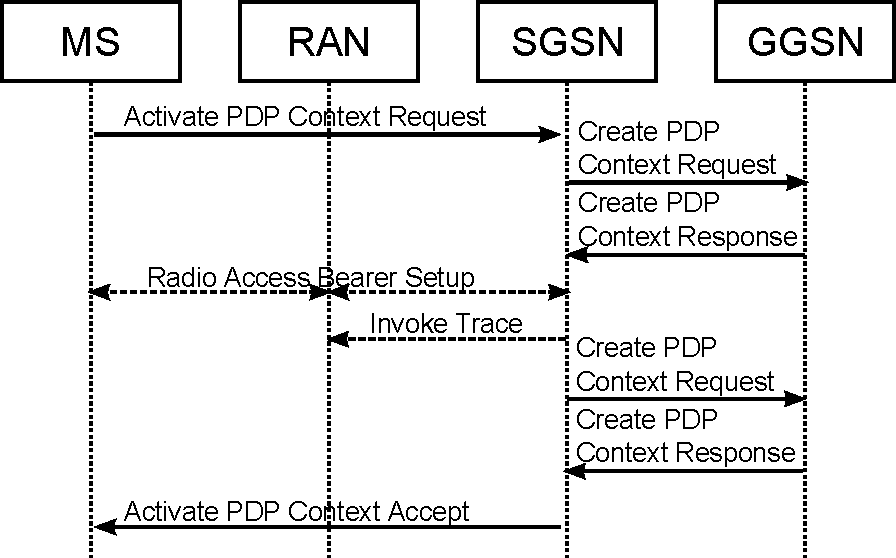
\includegraphics[width=0.8\columnwidth]{images/pdp-context-activation.pdf}
% 	\caption{PDP Context Activation Procedure in a UMTS network.}
% 	\label{c4:fig:pdpcontextactivation}
% \end{figure}



% \begin{itemize}
% \item 	Every bearer has a predefined QoS level between UE and P-GW.
% 		==> Level of Granularity for QoS control.
% \item	Initial bearer QoS level assigned by network based on subscription data.
% \item	Guaranteed Bit Rate (GBR) bearers: dedicated network resources permanently allocated at est/mod. Otherwise Non-GBR.
% \item	The Traffic Flow Template (TFT) belonging to a bearer is a set of packet filters that assign traffic flows to the bearer.
% \item	UL-TFT at UE, DL-TFT at \gls{PCEF} (P-GW).
% \item 	default bearer: always-on IP connectivity for the UE to a PDN
% \item	dedicated bearer:   
% 			\begin{itemize}
% 				\item any additional bearer for the same PDN
% 				\item \gls{TFT} associated with every ded. bearer
% 				\item establishment/modification decision only by \gls{EPC}
% 				\item QoS level assignment only by \gls{EPC}
% 			\end{itemize}

% \item	default bearer may be used as {m,c}atch-all traffic bearer for everything that does not match any filter
% \item	Every bearer associated with QCI and ARP.

% QoS class identifier (QCI): standardized scalar as reference for node-specific QoS parameters
% Allocation and Retention Policy (ARP): priority level preemption capability, preemption vulnerability.

% \item	All simultaneously active bearers by one UE are provided are provided by the same P-GW.
% \end{itemize}

% \begin{figure}[htb]
% 	\centering
% 	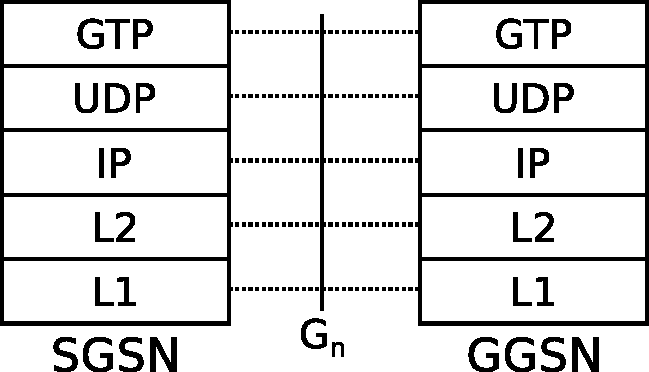
\includegraphics[width=0.6\columnwidth]{images/signalling-stack.pdf}
% 	\caption{Typical signaling protocol stack at the Gn interface between \gls{SGSN} and \gls{GGSN}.}
% 	\label{c4:fig:signallingstack}
% \end{figure}

% \begin{table}[htb]
% 	\caption{GTP header format (TODO: which one exactly. This looks like v2-U but should actually better be v1!)}
% 	\label{c4:tbl:gtpheader}
% 	\begin{tabu}{c|c|c|c|c|c|c|c|c|}
% 	\multicolumn{1}{c}{} & \multicolumn{8}{c}{\textbf{Bits}} \\
% 	\cline{2-9} \textbf{Octets} & 8 & 7 & 6 & 5 & 4 & 3 & 2 & 1 \\ 
% 	\cline{2-9} 1 & \multicolumn{3}{c|}{Version}  & P & T & Spare & Spare & Spare \\ 
% 	\cline{2-9} 2 & \multicolumn{8}{c|}{Message Type}  \\ 
% 	\cline{2-9} 3 & \multicolumn{8}{c|}{Message Length (1st Octet)}  \\ 
% 	\cline{2-9} 4 & \multicolumn{8}{c|}{Message Length (2nd Octet)}  \\ 
% 	\cline{2-9} m to & \multicolumn{8}{c|}{\multirow{2}{10cm}{If T flag is set to 1, then TEID shall be placed into octets 5-8. Otherwise, TEID field is not present at all.}} \\ 
% 	 k(m+3) & \multicolumn{8}{c|}{} \\ 
% 	\cline{2-9} n to (n+2) & \multicolumn{8}{c|}{Sequence Number} \\ 
% 	\cline{2-9} (n+3) & \multicolumn{8}{c|}{Spare} \\ 
% 	\cline{2-9} 
% 	\end{tabu} 
% \end{table}


%LTE: mention also \gls{PMIPv6} as \gls{gtp} alternative, and the option to have a combined \gls{SGW} \gls{PGW}


% request/response messaging
% response types:
% Possible context response types and which request types they answer:
% \begin{itemize}
% \item 192: ``non-existent'' UPDATE \& DELETE ONLY
% \item 193: ``invalid message format'' UPDATE \& DELETE ONLY
% \item 199: ``no resources available'' CREATE ONLY anywhere in the network to allocate context
% \item 200: ``service not supported'' UPDATE ONLY
% \item 201: ``mandatory IE incorrect''
% \item 202: ``mandatory IE missing''
% \item 204: ``system failure'' CREATE \& UPDATE ONLY
% \item 209: ``user authentication failed'' CREATE ONLY rejected for various reasons
% \end{itemize}

%---
%NSAPI {0;15} Integer
%linked \gls{NSAPI}: indicates the \gls{NSAPI} assigned to any one of the already activated \gls{PDP} contexts for this address/phone ("foreign key"?)

% TODO: convert to UMTS

% \begin{figure}[htb]
% 	\centering
% 	\includegraphics[width=1.0\textwidth]{images/UE-requested-PDN-connectivity.pdf}
% mdcm	\caption{\gls{PDN} connectivity request by the UE procedure sequence diagram.}
% 	\label{c4:fig:3gpp-uepdnreq}
% \end{figure}


%% creates
%IPv6 Stateless Address Autoconfiguration Procedure
%PDP Context Activation Procedure for A/Gb mode (additional (optional?) update pair)
%PDP Context Activation Procedure for Iu mode (additional (optional?) update pair)
%Secondary PDP Context Activation for Iu mode (additional (optional?) update pair)
%Secondary PDP Context Activation for A/Gb mode (additional (optional?) update pair)

%% deletes
%MS Initiated PDP Context Deactivation Procedure for A/Gb mode
%MS Initiated PDP Context Deactivation Procedure for Iu mode
%SGSN-initiated PDP Context Deactivation Procedure
%GGSN-initiated PDP Context Deactivation Procedure
%Combined GPRS/IMSI Attach Procedure (2x request+response, 1 to old, 1 to new)
%MS-Initiated Detach Procedure (1x request/response)
%Network-Initiated Detach Procedures (SGSN or HLR)


%% updates
%Inter SGSN Routeing Area Update (1x)
%Combined Inter SGSN RA/LA Update (1x)
%Iu mode RA Update Procedure (1x)
%SRNS Serving Radio Network Subsystem Relocation Procedure (1x)
%Combined Hard Handover and SRNS Relocation Procedure
%Combined Cell/URA (UTRAN Registration Area) Update and SRNS Relocation Procedure
%Enhanced Serving RNS Relocation
%Iu mode to A/Gb mode Intra SGSN Change
%Iu mode to A/Gb mode Inter SGSN Change
%A/Gb mode to Iu mode Inter SGSN Change
%SGSN-Initiated PDP Context Modification Procedure, A/Gb mode (2x pair (1 optional?))
%SGSN-Initiated PDP Context Modification Procedure, Iu mode (2x pair (1 optional?))
%GGSN-Initiated PDP Context Modification Procedure, Iu mode
%GGSN-Initiated PDP Context Modification Procedure, A/Gb mode
%MS-Initiated PDP Context Modification Procedure, A/Gb mode (2x, 1 optional/conditional)
%MS-Initiated PDP Context Modification Procedure, Iu mode (2x, 1 optional/conditional)
%PDP Context Activation Procedure for A/Gb mode (additional (optional?) update pair)
%PDP Context Activation Procedure for Iu mode (additional (optional?) update pair)
%Secondary PDP Context Activation for Iu mode (additional (optional?) update pair)
%Secondary PDP Context Activation for A/Gb mode (additional (optional?) update pair)
%RAB Release Procedure Using Gn/Gp (conditional if direct tunnel and context to be preserved)
%Iu Release Procedure Using Gn/Gp (conditional if direct tunnel and context to be preserved)
%RAB Assignment Procedure Using Gn/Gp (conditional direct tunnel)

%%%%%%%%%%%%%%%%%%%%%%%%%%%%%%%%%%%%%%%%%%%%%%%%%%%%%%%%%%%%%%%%%%%%%%%%%%%%%%%%
%%!TEX root = dissertation.tex
%%%%%%%%%%%%%%%%%%%%%%%%%%%%%%%%%%%%%%%%%%%%%%%%%%%%%%%%%%%%%%%%%%%%%%%%%%%%%%%%
%
% Collection of all relevant mobile radio specifications and descriptions
%
\section{Übersicht}

\begin{itemize}
\item Einarbeitung
	\begin{itemize}
		\item Architektur von 3G-Netzen
		\item Modelle zur Beschreibung von Datenverkehrsflüssen
		\item Einarbeitung in das Messsystem des FTW
	\end{itemize}
\item Definition eines einfachen Bearer-Modells
\item Programmierung der Auswertung
\item Durchführung und Auswertung der Messungen
\item Anfertigung eines Berichtes
\end{itemize}

\section{Modeling}
Macroscopic Behavior

	-- time Connection Setup until Call Termination with Talk Spurts
	--> ON/OFF Process
	--> Empricial measurement
	
Source Traffic Model
	-- 2 parts: 
		arrival process for user activities
		process describing activity phase
	-- arrival time:
		User begins web browsing
	
Simulation \& Software
	ns-2 UMTS mobile parts only
	ns-3 GSoC2010 implementing \ac{UTRAN} (MAC\&PHY) incl radio bearers (+OpenFlow)
	Harald Welte GPRS: OpenBSC, OpenGGSN incl GTP
	

EPS first introduced in 3GPP Release 8, completed in March 2009. Consisting of EUTRAN, EPC (formerly SAE)


	


\begin{figure}[htbp]
 \centering
 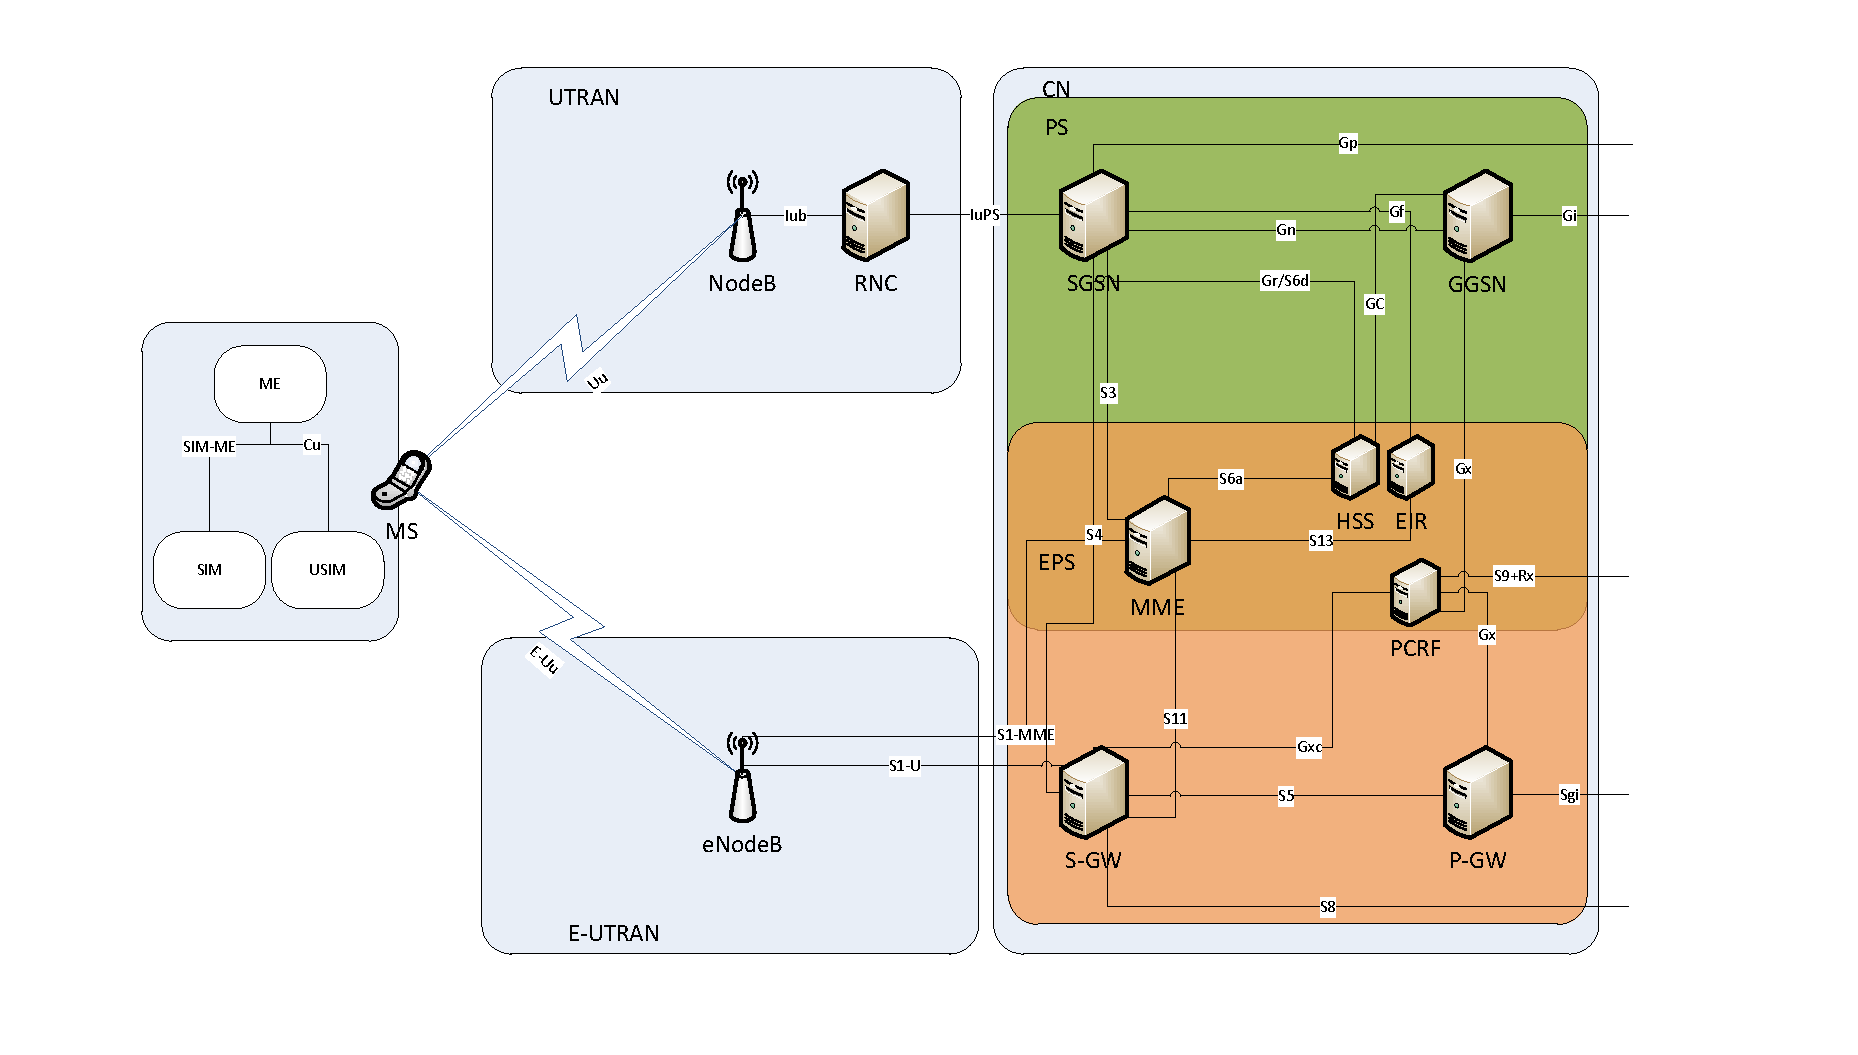
\includegraphics[width=1.0\textwidth]{images/3gpp/eps_ps-overview.pdf}
 \caption{Beispielnetz}\label{fig:netzwerk2}
\end{figure}

List of interfaces in the 3G/LTE PS network
\begin{itemize}
\item \textbf{Uu}: Interface between the mobile station (MS) and the fixed network part in Iu mode. The Uu interface is the Iu mode network interface for providing packet data services over the radio to the MS. The MT part of the MS is used to access the UMTS services through this interface.
\item \textbf{Iub}: Interface between a NodeB and a RNC.
\item \textbf{IuPS}: Interface between a RNC and a SGSN.

\item \textbf{S1-U}: Interface between a eNodeB and a S-GW. User plane bearer tunneling.
\item \textbf{S1-MME}: Interface between a eNodeB and a MME.
\item \textbf{S3}: Interface between a SGSN and a MME. User/bearer information exchange for active/idle state 3g network access mobility.
\item \textbf{S4}: Interface between a SGSN and a S-GW.	 2G user plane tunneling. GPRS mobility and control.
\item \textbf{S5}: Interface between a S-GW and a P-GW within the same PLMN. User plane tunneling; S-GW relocation due to mobility.
\item \textbf{S6a}: Interface between a MME and a HSS. Auth/auth data transfer to evolved system.
\item \textbf{Gr/S6d}: Interface between a SGSN and a HSS. 
\item \textbf{S8}: Interface between a S-GW and a P-GW in different PLMNs. Inter-PLMN variant to S5.
\item \textbf{S9}: Interface between a PRCF and the packet data network. Data exchange to visited PCRF PLMN.
\item \textbf{S11}: Interface between a S-GW and a MME.
\item \textbf{S12}: UTRAN to S-GW reference point. Based on Iu-u/Gn-u. Direct Tunnel via GTP-U.
\item \textbf{S13}: Interface between a MME and a EIR. UE identity check.
\item \textbf{SGi}: The reference point between the EPC based PLMN and the packet data network. Same as Gi for 3gpp.

\item \textbf{GC}: Interface between a HSS and a GGSN.
\item \textbf{Gf}: Interface between a SGSN and a EIR.
\item \textbf{Gi}: Reference point between Packet Domain and an external packet data network.
\item \textbf{Gn}: Interface between two GSNs within the same PLMN.
\item \textbf{Gp}: Interface between two GSNs in different PLMNs. The Gp interface allows support of Packet Domain network services across areas served by the co-operating PLMNs.
\item \textbf{Gx}: Interface between a PCRF and a P-GW/GGSN. QoS policy and charging rules transfer.
\item \textbf{Gxc}: Interface between a PCRF and a S-GW.

\item \textbf{Rx}: Interface between a PRCF and the packet data network.
\end{itemize}

\section{Control Plane Protocol Stacks}

\begin{figure}[htbp]
 \centering
 \includegraphics[width=1.0\textwidth]{images/3gpp/eNB-MME-layers.pdf}
 \caption{Beispielnetz}\label{fig:3gpp-enbmme}
\end{figure}

\begin{figure}[htbp]
 \centering
 \includegraphics[width=1.0\textwidth]{images/3gpp/SGSN-MME-layers.pdf}
 \caption{Beispielnetz}\label{fig:3gpp-sgsnmme}
\end{figure}

\begin{figure}[htbp]
 \centering
 \includegraphics[width=1.0\textwidth]{images/3gpp/S-GW-P-GW-layers.pdf}
 \caption{Beispielnetz}\label{fig:3gpp-sgwpgw}
\end{figure}

\begin{figure}[htbp]
 \centering
 \includegraphics[width=1.0\textwidth]{images/3gpp/MME-S-GW-layers.pdf}
 \caption{Beispielnetz}\label{fig:3gpp-mmesgw}
\end{figure}


\begin{figure}[htbp]
 \centering
 \includegraphics[width=1.0\textwidth]{images/3gpp/3g-userplane.pdf}
 \caption{Beispielnetz}\label{fig:3gpp-umtsuserplane}
\end{figure}

\begin{figure}[htbp]
 \centering
 \includegraphics[width=1.0\textwidth]{images/3gpp/LTE-userplane.pdf}
 \caption{Beispielnetz}\label{fig:3gpp-lteuserplane}
\end{figure}


\section{Bearers}

As you said only 11 bearer are permitted.
So PDN connection(Default bearer) + Dedicated bearers put together should not exceed 11 bearers at any instant of time at UE side.
Theoretically 11 PDN connections are possible. But i dont think it will be of any use in practical EPS topology.

One UE Can have Maximum 3 PDN connection.
where as my knowledge is concern one UE can support maximum 11 bearers, 3 default and 8 dedicated bearers.

Does I will get in any spec for this. As the default bearer are of  NON-GBR type and and there are 5-9 are of NON-GBR QCI so I think a ue can have maximum 5 default bearer If two default bearer can not use same QCI.

\begin{figure}[htbp]
 \centering
 \includegraphics[width=1.0\textwidth]{images/3gpp/bearers.pdf}
 \caption{Beispielnetz}\label{fig:3gpp-bearers}
\end{figure}


\begin{figure}[htbp]
 \centering
 \includegraphics[width=1.0\textwidth]{images/3gpp/ECM-states.pdf}
 \caption{Beispielnetz}\label{fig:3gpp-ecmstates}
\end{figure}

\begin{itemize}
\item 	Every bearer has a predefined QoS level between UE and P-GW.
		==> Level of Granularity for QoS control.
\item	Initial bearer QoS level assigned by network based on subscription data.
\item	Guaranteed Bit Rate (GBR) bearers: dedicated network resources permanently allocated at est/mod. Otherwise Non-GBR.
\item	The Traffic Flow Template (TFT) belonging to a bearer is a set of packet filters that assign traffic flows to the bearer.
\item	UL-TFT at UE, DL-TFT at PCEF (P-GW).
\item 	default bearer: always-on IP connectivity for the UE to a PDN
\item	dedicated bearer:   
			\begin{itemize}
				\item any additional bearer for the same PDN
				\item Traffic Flow Template (TFT) associated with every ded. bearer
				\item establishment/modification decision only by EPC
				\item QoS level assignment only by EPC
			\end{itemize}

\item	default bearer may be used as {m,c}atch-all traffic bearer for everything that does not match any filter
\item	Every bearer associated with QCI and ARP.

QoS class identifier (QCI): standardized scalar as reference for node-specific QoS parameters
Allocation and Retention Policy (ARP): priority level preemption capability, preemption vulnerability.

\item	All simultaneously active bearers by one UE are provided are provided by the same P-GW.
\end{itemize}

EMM Service request procedure

\begin{figure}[htbp]
 \centering
 \includegraphics[width=1.0\textwidth]{images/3gpp/UE-service-request.pdf}
 \caption{Beispielnetz}\label{fig:3gpp-ueservicereq}
\end{figure}

Annotations:
1. Encapsulated in RRC message.
2. Forwarded in S1-AP Initial UE Message.
3. Various security procedures.


\section{Information Storage}
per PLMN node, cf. 3GPP TS 23.401 clause 5.7.

\begin{figure}[htbp]
 \centering
 \includegraphics[width=1.0\textwidth]{images/3gpp/UE-requested-PDN-connectivity.pdf}
 \caption{Beispielnetz}\label{fig:3gpp-uepdnreq}
\end{figure}


\section{GTP}
\subsection{GTPv2}



\begin{tabular}{c|c|c|c|c|c|c|c|c|}
\multicolumn{1}{c}{} & \multicolumn{8}{c}{\textbf{Bits}} \\
\cline{2-9} \textbf{Octets} & 8 & 7 & 6 & 5 & 4 & 3 & 2 & 1 \\ 
\cline{2-9} 1 & \multicolumn{3}{c|}{Version}  & P & T & Spare & Spare & Spare \\ 
\cline{2-9} 2 & \multicolumn{8}{c|}{Message Type}  \\ 
\cline{2-9} 3 & \multicolumn{8}{c|}{Message Length (1st Octet)}  \\ 
\cline{2-9} 4 & \multicolumn{8}{c|}{Message Length (2nd Octet)}  \\ 
\cline{2-9} m to & \multicolumn{8}{c|}{\multirow{2}{10cm}{If T flag is set to 1, then TEID shall be placed into octets 5-8. Otherwise, TEID field is not present at all.}} \\ 
 k(m+3) & \multicolumn{8}{c|}{} \\ 
\cline{2-9} n to (n+2) & \multicolumn{8}{c|}{Sequence Number} \\ 
\cline{2-9} (n+3) & \multicolumn{8}{c|}{Spare} \\ 
\cline{2-9} 
\end{tabular} 
\subsection{GTP-C}

\begin{tabular}{c|c|c|c|c|c|c|c|c|}
\multicolumn{1}{c}{} & \multicolumn{8}{c}{\textbf{Bits}} \\
\cline{2-9} \textbf{Octets} & 8 & 7 & 6 & 5 & 4 & 3 & 2 & 1 \\ 
\cline{2-9} 1 & \multicolumn{3}{c|}{Version}  & P & T=1 & Spare & Spare & Spare \\ 
\cline{2-9} 2 & \multicolumn{8}{c|}{Message Type}  \\ 
\cline{2-9} 3 & \multicolumn{8}{c|}{Message Length (1st Octet)}  \\ 
\cline{2-9} 4 & \multicolumn{8}{c|}{Message Length (2nd Octet)}  \\ 
\cline{2-9} 5 & \multicolumn{8}{c|}{Tunnel Endpoint Identifier (1st Octet)} \\ 
\cline{2-9} 6 & \multicolumn{8}{c|}{Tunnel Endpoint Identifier (2nd Octet)} \\ 
\cline{2-9} 7 & \multicolumn{8}{c|}{Tunnel Endpoint Identifier (3rd Octet)} \\ 
\cline{2-9} 8 & \multicolumn{8}{c|}{Tunnel Endpoint Identifier (4th Octet)} \\ 
\cline{2-9} 9 & \multicolumn{8}{c|}{Sequence Number (1st Octet)} \\
\cline{2-9} 10 & \multicolumn{8}{c|}{Sequence Number (2nd Octet)} \\
\cline{2-9} 11 & \multicolumn{8}{c|}{Sequence Number (3rd Octet)} \\
\cline{2-9} 12 & \multicolumn{8}{c|}{Spare} \\
\cline{2-9}
\end{tabular} 

12 Byte GTPv2-C header.

\subsubsection{Create Session Request Message}

Information Elements Table for PDP Context Activation Case only

\begin{longtabu}{|p{2cm}|c|p{1.5cm}|p{8cm}|}
\hline
Information Element 						& IE Type 					& Max Wire Size (Bytes)	& Comment \\ \hline
IMSI 										& IMSI 						& 12					& \\ \hline
MSISDN 										& MSISDN					& 12					& On S11 Interface if provided by HSS; In case of UE requested connectivity if MME has it stored. \\ \hline
MEI Identity 								& MEI 						& 12					& If available at MME. \\ \hline
User Location Information 					& ULI						& 						& E-UTRAN initial attach \&  UE requested connectivity only; included by S-GW if received from MME via S5/S8; included on S4 and S5/S8 for PDP context activation, either CGI, SAI, or RAI. \\ \hline
Serving Network								& Serving Network			& 						& Initial E-UTRAN attach, context activation and UE requested connectivity \\ \hline
RAT Type									& RAT Type					& 5						& \\ \hline
Indication Flags							& Indication				& 6						& Flags: S5/S8 Protocol Type; Dual Address Bearer Flag; Handover Indication; Direct Tunnel Flag; Piggybacking Supported; Change Reporting Support Indication \\ \hline
Sender F-TEID for Control Plane				& F-TEID					& 						& \\ \hline
P-G S5/S8 Address for Control Plane or PMIP	& F-TEID					& 						& On S11/S4 interfaces; 0 if initial attach, context activation or PDN connectivity \\ \hline
Access Point Name							& APN						& 83					& \\ \hline
Selection Mode								& Selection Mode			& 						& Indicate whether subscribed or non-subscribed, chosen by MME, was selected \\ \hline
PDN Type									& PDN Type					& 						& IPv4, IPv6 or IPv4v6. \\ \hline
PDN Address Allocation						& PAA						& 26					& Set to static IP address; else (dynamic) to 0.0.0.0 or IPv6 Prefix Length 0. \\ \hline
Maximum APN Restriction						& APN Restriction			& 						& Set to most stringent restriction of any active bearer. \\ \hline
Aggregate Maximum Bit Rate					& ABMR						& 12					& \\ \hline
Protocol Configuration Options				& PCO						& 254					& Forwarded from UE to P-GW via S-GW via MME. \\ \hline
Bearer Contexts to be created				& Bearer Context			& 						& present multiple times to represent list of bearers \\ \hline
Trace Information							& Trace Information 		& 						& If S-GW / P-GW is activated. \\ \hline
Recovery									& Recovery					& 5						& If peer node contacted for the first time. \\ \hline
MME-FQ-CSID									& FQ-CSID					& 						& Included by MME on S11 \\ \hline
SGW-FQ-CSID									& FQ-CSID					& 						& Included by S-GW on S5/S8 \\ \hline
UE Time Zone								& UE Time Zone 				& 						& Can be included by MME on S11; forwarded to P-GW via S-GW \\ \hline
User CSG Information						& UCI						& 						& If UE accessed via CSG cell or hybrid cell \\ \hline
Charging Characteristics					& Charging Characteristics	&						& \\ \hline
Private Extensions							& Private Extensions		&						& \\ \hline

\end{longtabu}

\subsubsection{Information Elements Wire Format}

\paragraph{IMSI}

\begin{tabular}{c|p{1cm}|p{1cm}|p{1cm}|p{1cm}|p{1cm}|p{1cm}|p{1cm}|p{1cm}|}
\multicolumn{1}{c}{} & \multicolumn{8}{c}{\textbf{Bits}} \\
\cline{2-9} \textbf{Octets} & 8 & 7 & 6 & 5 & 4 & 3 & 2 & 1 \\ 
\cline{2-9} 1 & \multicolumn{8}{c|}{Type = 1 (decimal)} \\ 
\cline{2-9} 2 to 3 & \multicolumn{8}{c|}{Length = n}  \\ 
\cline{2-9} 4 & \multicolumn{4}{c|}{Spare} & \multicolumn{4}{c|}{Instance} \\ 
\cline{2-9} 5 & \multicolumn{4}{c|}{Number digit 2} & \multicolumn{4}{c|}{Number digit 1} \\ 
\cline{2-9} 6 & \multicolumn{4}{c|}{Number digit 4} & \multicolumn{4}{c|}{Number digit 3} \\ 
\cline{2-9} ... & \multicolumn{4}{c|}{...} & \multicolumn{4}{c|}{...} \\ 
\cline{2-9} n+4 & \multicolumn{4}{c|}{Number digit m} & \multicolumn{4}{c|}{Number digit m-1} \\ 
\cline{2-9}
\end{tabular} 

Decimals coded as TBCD; if odd number fill last nibble with 1; max digits is 15.\\
Max IE size 12 Byte.

\paragraph{APN}

\begin{tabular}{c|p{1cm}|p{1cm}|p{1cm}|p{1cm}|p{1cm}|p{1cm}|p{1cm}|p{1cm}|}
\multicolumn{1}{c}{} & \multicolumn{8}{c}{\textbf{Bits}} \\
\cline{2-9} \textbf{Octets} & 8 & 7 & 6 & 5 & 4 & 3 & 2 & 1 \\ 
\cline{2-9} 1 & \multicolumn{8}{c|}{Type = 71 (decimal)} \\ 
\cline{2-9} 2 to 3 & \multicolumn{8}{c|}{Length = n}  \\ 
\cline{2-9} 4 & \multicolumn{4}{c|}{Spare} & \multicolumn{4}{c|}{Instance} \\ 
\cline{2-9} 5 to (n+4) & \multicolumn{8}{c|}{Access Point Name} \\ 
\cline{2-9}
\end{tabular} 

Full APN name including APN Network Identifier and APN Operator Identifier.
Network Identifier: max length 63 bytes.
Operator Identifier: mnc<3digits>.mcc<3digits>.gprs; 16 bytes (18 incl dots).
(Ex: ggsn-cluster-A.provinceB.mnc012.mcc345.gprs)

Max total $4+63+16=83$

\paragraph{AMBR}

\begin{tabular}{c|p{1cm}|p{1cm}|p{1cm}|p{1cm}|p{1cm}|p{1cm}|p{1cm}|p{1cm}|}
\multicolumn{1}{c}{} & \multicolumn{8}{c}{\textbf{Bits}} \\
\cline{2-9} \textbf{Octets} & 8 & 7 & 6 & 5 & 4 & 3 & 2 & 1 \\ 
\cline{2-9} 1 & \multicolumn{8}{c|}{Type = 72 (decimal)} \\ 
\cline{2-9} 2 to 3 & \multicolumn{8}{c|}{Length = n}  \\ 
\cline{2-9} 4 & \multicolumn{4}{c|}{Spare} & \multicolumn{4}{c|}{Instance} \\ 
\cline{2-9} 5 to 8 & \multicolumn{8}{c|}{APN-AMBR for uplink} \\ 
\cline{2-9} 9 to 12 & \multicolumn{8}{c|}{APN-AMBR for downlink} \\ 
\cline{2-9}
\end{tabular} 


Total size 12 bytes.


\paragraph{Recovery}

\begin{tabular}{c|p{1cm}|p{1cm}|p{1cm}|p{1cm}|p{1cm}|p{1cm}|p{1cm}|p{1cm}|}
\multicolumn{1}{c}{} & \multicolumn{8}{c}{\textbf{Bits}} \\
\cline{2-9} \textbf{Octets} & 8 & 7 & 6 & 5 & 4 & 3 & 2 & 1 \\ 
\cline{2-9} 1 & \multicolumn{8}{c|}{Type = 3 (decimal)} \\ 
\cline{2-9} 2 to 3 & \multicolumn{8}{c|}{Length = n}  \\ 
\cline{2-9} 4 & \multicolumn{4}{c|}{Spare} & \multicolumn{4}{c|}{Instance} \\ 
\cline{2-9} 5 to (n+4) & \multicolumn{8}{c|}{Recovery (Restart Counter} \\ 
\cline{2-9}
\end{tabular} 

IN GTPv2 first release IE length is 5 bytes. May be longer in the future.


\paragraph{MEI}

\begin{tabular}{c|p{1cm}|p{1cm}|p{1cm}|p{1cm}|p{1cm}|p{1cm}|p{1cm}|p{1cm}|}
\multicolumn{1}{c}{} & \multicolumn{8}{c}{\textbf{Bits}} \\
\cline{2-9} \textbf{Octets} & 8 & 7 & 6 & 5 & 4 & 3 & 2 & 1 \\ 
\cline{2-9} 1 & \multicolumn{8}{c|}{Type = 75 (decimal)} \\ 
\cline{2-9} 2 to 3 & \multicolumn{8}{c|}{Length = n}  \\ 
\cline{2-9} 4 & \multicolumn{4}{c|}{Spare} & \multicolumn{4}{c|}{Instance} \\ 
\cline{2-9} 5 to (n+4) & \multicolumn{8}{c|}{Mobile Equipment (ME) Identity} \\ 
\cline{2-9}
\end{tabular} 

15 (IMEI) or 16 (IMEISV) BCD digits filled with 1 to full octet. Size is 12 bytes.

\paragraph{MSISDN}

\begin{tabular}{c|p{1cm}|p{1cm}|p{1cm}|p{1cm}|p{1cm}|p{1cm}|p{1cm}|p{1cm}|}
\multicolumn{1}{c}{} & \multicolumn{8}{c}{\textbf{Bits}} \\
\cline{2-9} \textbf{Octets} & 8 & 7 & 6 & 5 & 4 & 3 & 2 & 1 \\ 
\cline{2-9} 1 & \multicolumn{8}{c|}{Type = 76 (decimal)} \\ 
\cline{2-9} 2 to 3 & \multicolumn{8}{c|}{Length = n}  \\ 
\cline{2-9} 4 & \multicolumn{4}{c|}{Spare} & \multicolumn{4}{c|}{Instance} \\ 
\cline{2-9} 5 & \multicolumn{4}{c|}{Number digit 2} & \multicolumn{4}{c|}{Number digit 1} \\ 
\cline{2-9} 6 & \multicolumn{4}{c|}{Number digit 4} & \multicolumn{4}{c|}{Number digit 3} \\ 
\cline{2-9} ... & \multicolumn{4}{c|}{...} & \multicolumn{4}{c|}{...} \\ 
\cline{2-9} n+4 & \multicolumn{4}{c|}{Number digit m} & \multicolumn{4}{c|}{Number digit m-1} \\ 
\cline{2-9}
\end{tabular} 

MSISDN limited to 15 digits. Max total size 12 bytes.


\paragraph{Indication}
\centering
\begin{tabular}{c|p{1cm}|p{1cm}|p{1cm}|p{1cm}|p{1cm}|p{1cm}|p{1cm}|p{1cm}|}
\multicolumn{1}{c}{} & \multicolumn{8}{c}{\textbf{Bits}} \\
\cline{2-9} \textbf{Octets} & 8 & 7 & 6 & 5 & 4 & 3 & 2 & 1 \\ 
\cline{2-9} 1 & \multicolumn{8}{c|}{Type = 77 (decimal)} \\ 
\cline{2-9} 2 to 3 & \multicolumn{8}{c|}{Length = n}  \\ 
\cline{2-9} 4 & \multicolumn{4}{c|}{Spare} & \multicolumn{4}{c|}{Instance} \\ 
\cline{2-9} 5 & DAF & DTF & HI & DFI & OI & ISRSI & ISRAI & SGWCI \\ 
\cline{2-9} 6 & Spare & UIMSI & CFSI & CRSI & P & PT & SI & MSV \\ 
\cline{2-9} 7 to (n+4) & \multicolumn{8}{c|}{These octet(s) is/are present only if explicitly specified} \\ 
\cline{2-9}
\end{tabular} 

Size is 7 bytes.

\paragraph{PCO}
\centering
\begin{tabular}{c|p{1cm}|p{1cm}|p{1cm}|p{1cm}|p{1cm}|p{1cm}|p{1cm}|p{1cm}|}
\multicolumn{1}{c}{} & \multicolumn{8}{c}{\textbf{Bits}} \\
\cline{2-9} \textbf{Octets} & 8 & 7 & 6 & 5 & 4 & 3 & 2 & 1 \\ 
\cline{2-9} 1 & \multicolumn{8}{c|}{Type = 78 (decimal)} \\ 
\cline{2-9} 2 to 3 & \multicolumn{8}{c|}{Length = n}  \\ 
\cline{2-9} 4 & \multicolumn{4}{c|}{Spare} & \multicolumn{4}{c|}{Instance} \\ 
\cline{2-9} 5 to (n+4) & \multicolumn{8}{c|}{Protocol Configuration Options} \\
\cline{2-9}
\end{tabular} 

Minimum length 4+3-3, maximum length 4+253-3; average?


\paragraph{PAA}
\centering

\begin{tabular}{c|p{1cm}|p{1cm}|p{1cm}|p{1cm}|p{1cm}|p{1cm}|p{1cm}|p{1cm}|}
\multicolumn{1}{c}{} & \multicolumn{8}{c}{\textbf{Bits}} \\
\cline{2-9} \textbf{Octets} & 8 & 7 & 6 & 5 & 4 & 3 & 2 & 1 \\ 
\cline{2-9} 1 & \multicolumn{8}{c|}{Type = 79 (decimal)} \\ 
\cline{2-9} 2 to 3 & \multicolumn{8}{c|}{Length = n}  \\ 
\cline{2-9} 4 & \multicolumn{4}{c|}{Spare} & \multicolumn{4}{c|}{Instance} \\ 
\cline{2-9} 5 & \multicolumn{5}{c|}{Spare} & \multicolumn{3}{c|}{PDN Type} \\
\cline{2-9} 6 to (n+4) & \multicolumn{8}{c|}{PDN Adress and Prefix} \\
\cline{2-9}
\end{tabular} 

Either 9 (IPv4), 22 (IPv6), or 26 (IPv4v6).


\paragraph{RAT Type}
\centering
\begin{tabular}{c|p{1cm}|p{1cm}|p{1cm}|p{1cm}|p{1cm}|p{1cm}|p{1cm}|p{1cm}|}
\multicolumn{1}{c}{} & \multicolumn{8}{c}{\textbf{Bits}} \\
\cline{2-9} \textbf{Octets} & 8 & 7 & 6 & 5 & 4 & 3 & 2 & 1 \\ 
\cline{2-9} 1 & \multicolumn{8}{c|}{Type = 82 (decimal)} \\ 
\cline{2-9} 2 to 3 & \multicolumn{8}{c|}{Length = n}  \\ 
\cline{2-9} 4 & \multicolumn{4}{c|}{Spare} & \multicolumn{4}{c|}{Instance} \\ 
\cline{2-9} 5 & \multicolumn{8}{c|}{RAT Type} \\
\cline{2-9} 6 to (n+4) & \multicolumn{8}{c|}{These octet(s) is/are present only if explicitly specified} \\
\cline{2-9}
\end{tabular} 

Maximum length 5 to ?.

\paragraph{Serving Network}

\centering
\begin{tabular}{c|p{1cm}|p{1cm}|p{1cm}|p{1cm}|p{1cm}|p{1cm}|p{1cm}|p{1cm}|}
\multicolumn{1}{c}{} & \multicolumn{8}{c}{\textbf{Bits}} \\
\cline{2-9} \textbf{Octets} & 8 & 7 & 6 & 5 & 4 & 3 & 2 & 1 \\ 
\cline{2-9} 1 & \multicolumn{8}{c|}{Type = 83 (decimal)} \\ 
\cline{2-9} 2 to 3 & \multicolumn{8}{c|}{Length = n}  \\ 
\cline{2-9} 4 & \multicolumn{4}{c|}{Spare} & \multicolumn{4}{c|}{Instance} \\ 
\cline{2-9} 5 & \multicolumn{4}{c|}{MCC digit 2} & \multicolumn{4}{c|}{MCC digit 1} \\ 
\cline{2-9} 6 & \multicolumn{4}{c|}{MNC digit 3} & \multicolumn{4}{c|}{MCC digit 3} \\ 
\cline{2-9} 7 & \multicolumn{4}{c|}{MNC digit 2} & \multicolumn{4}{c|}{MNC digit 1} \\ 
\cline{2-9} 8 to (n+4) & \multicolumn{8}{c|}{These octet(s) is/are present only if explicitly specified} \\
\cline{2-9}
\end{tabular} 

Maximum length 7 to ?.


\paragraph{User Location Information}

\centering
\begin{tabular}{c|p{1cm}|p{1cm}|p{1cm}|p{1cm}|p{1cm}|p{1cm}|p{1cm}|p{1cm}|}
\multicolumn{1}{c}{} & \multicolumn{8}{c}{\textbf{Bits}} \\
\cline{2-9} \textbf{Octets} & 8 & 7 & 6 & 5 & 4 & 3 & 2 & 1 \\ 
\cline{2-9} 1 & \multicolumn{8}{c|}{Type = 86 (decimal)} \\ 
\cline{2-9} 2 to 3 & \multicolumn{8}{c|}{Length = n}  \\ 
\cline{2-9} 4 & \multicolumn{4}{c|}{Spare} & \multicolumn{4}{c|}{Instance} \\ 
\cline{2-9} 5 & \multicolumn{3}{c|}{Spare} & ECGI & TAI & RAI & SAI & CGI \\ 
\cline{2-9} a to a+6 & \multicolumn{8}{c|}{CGI} \\ 
\cline{2-9} 7 & \multicolumn{8}{c|}{SAI} \\ 
\cline{2-9} 7 & \multicolumn{8}{c|}{RAI} \\ 
\cline{2-9} 7 & \multicolumn{8}{c|}{TAI} \\ 
\cline{2-9} 7 & \multicolumn{8}{c|}{ECGI} \\ 
\cline{2-9} 8 to (n+4) & \multicolumn{8}{c|}{These octet(s) is/are present only if explicitly specified} \\
\cline{2-9}
\end{tabular} 


\subsection{GTP-U}



% \begin{multicols}{2}
% \setbox\ltmcbox\vbox{
% \makeatletter\col@number\@ne
% 	\begin{longtabu}{|X[2.5]|X[1.2]|X[0.7]|} \hline
% 		\textbf{\gls{IE}} & \textbf{Presence} & \textbf{Size}\\ \hline
% 		\gls{IMSI} & cond. & \SI{8}{\byte} \\ \hline
% 		\acrshort{RAI} & opt. & \SI{6}{\byte} \\ \hline
% 		Recovery & opt. & \SI{1}{\byte} \\ \hline
% 		Selection mode	& cond. & \SI{1}{\byte} \\ \hline
% 		\gls{TEID} Data I & mand. & \SI{4}{\byte} \\ \hline
% 		\gls{TEID} Control Plane & cond. & \SI{4}{\byte} \\ \hline
% 		\gls{NSAPI} & mand. & \SI{1}{\byte} \\ \hline
% 		Linked \gls{NSAPI} & cond. & \SI{1}{\byte} \\ \hline
% 		Charging Characteristics & cond. & \SI{2}{\byte} \\ \hline
% 		Trace Reference & opt. & \SI{2}{\byte} \\ \hline
% 		Trace Type & opt. & \SI{2}{\byte} \\ \hline
% 		End User Address & cond. & \SI{8}{\byte} \\ \hline
% 		\gls{APN} & cond. & max \SI{102}{\byte} \\ \hline % APN format defined in 23.003 section 9
% 		\acrshort{PCO} & opt. & max \SI{255}{\byte} \\ \hline % defined in 24.008 section 10.5.6.3
% 		\gls{SGSN} signaling address & mand.  & \SI{6}{\byte} \\ \hline % defined in 23.003 section 5 (without address type and length fields)
% 		\gls{SGSN} user traffic address & mand. & \SI{6}{\byte} \\ \hline % same as above
% 		\gls{MSISDN} & cond. & max \SI{17}{\byte} \\ \hline % ITU-T E.164 msisdn format recommendation of max 15 chars
% 		\gls{QoS} Profile & mand. & max \SI{257}{\byte} \\ \hline
% 		\gls{TFT} & cond. & max \SI{257}{\byte} \\ \hline % defined in 24.008 section 10.5.6.12
% 		 Trigger Id & opt. & var. \\ \hline % no definition found
% 		 \acrshort{OMC} Identity & opt. & var. \\ \hline % maybe in MAP 29.002, however not further definition found
% 		 Common Flags & opt. & \SI{3}{\byte} \\ \hline
% 		 \gls{APN} Restriction & opt. & \SI{3}{\byte} \\ \hline
% 		 \gls{RAT} & opt. & \SI{3}{\byte} \\ \hline
% 		 User Location Information & opt. & \SI{10}{\byte} \\ \hline
% 		 \gls{MS} Time Zone & opt. & \SI{4}{\byte} \\ \hline
% 		 \gls{IMEI}(\acrshort{SV}) & cond. & \SI{10}{\byte} \\ \hline
% 		 \gls{CAMEL} Charging Information Container & opt. & var. \\ \hline
% 		 Additional Trace Info & opt. & \SI{11}{\byte} \\ \hline
% 		 Correlation-ID & opt. & \SI{3}{\byte} \\ \hline
% 		 Evolved Allocation Retention Priority I & opt. & \SI{3}{\byte} \\ \hline
% 		 Extended Common Flags & opt. & \SI{3}{\byte} \\ \hline % might be more, but seems unused 
% 		 User \acrshort{CSG} Information & opt. & \SI{10}{\byte} \\ \hline
% 		 \gls{APN}-\acrshort{AMBR} & opt.  & \SI{11}{\byte} \\ \hline
% 		 Signaling Priority Indication & opt. & \SI{3}{\byte} \\ \hline % might be more, but seems unused
% 		 Private Extension & opt. & var. \\ \hline
% 	\end{longtabu}
% \unskip
% \unpenalty
% \unpenalty}

% \unvbox\ltmcbox

% \end{multicols}